% drift_makalesi.tex — iki-sütunlu makale taslağı (revtex KULLANMADAN)
% Derleme: pdflatex drift_makalesi.tex  (iki kez, referanslar için)
% Şekiller bu dosyayla aynı dizinde (drift_monitor/) PNG olarak bulunmalı;
% üretim: python3 make_figures.py ; python3 make_fig5_architecture.py
\documentclass[twocolumn,a4paper,10pt]{article}

\usepackage[T1]{fontenc}
\usepackage[utf8]{inputenc}
\usepackage{lmodern}
\usepackage{amsmath,amssymb}
\usepackage{graphicx}
\usepackage{booktabs}
\usepackage{textcomp}
\usepackage[hidelinks,unicode]{hyperref}
\usepackage{geometry}
\geometry{margin=2cm}

% Şekiller bu dizinde
\graphicspath{{./}}

\title{\bfseries Dondurulmuş-spin proton EDM halkasında kapalı-yörünge
tabanlı hizalama drift izlemesi: performans ve gözlenebilirlik
sınırları\thanks{Taslak v0.1 (2026-06-19). \texttt{makale-taslagi-2.md} ve
\texttt{drift\_monitor/} test sonuçlarından konsolide edilmiştir; başlık
geçicidir.}}

\author{(yazar bilgisi)}
\date{\today}

\begin{document}
\maketitle

\begin{abstract}
\noindent
Proton EDM (pEDM) deneyinin alternating-gradient (AG) versiyonunda, manyetik
kuadrupol hizalama hataları baskın sistematik kaynağıdır ve spin koherans
zaman ölçeğinde $\sim 10\,\mu$m seviyesinde kontrol altında tutulmalıdır
\cite{omarov2022}. Bu çalışmada, bu hizalamayı sürekli izlemek için kalibrasyon
anına göreli bir \emph{kapalı-yörünge tabanlı online hizalama drift izleme
yöntemi} öneriyor ve sistematik simülasyon testleriyle hem yeteneklerini hem de
gözlenebilirlik sınırını niceliyoruz. Yaklaşım, problemi bilinçli olarak yeniden
tanımlar: amaç
\emph{mutlak hizalama rekonstrüksiyonu} ($\Delta q = R^{-1}\mathbf{y}$) değil,
\emph{göreli hizalama kararlılığı izlemesi}dir. Yöntem, kalibrasyon anındaki
BPM okumasını referans alarak
$\widehat{\delta q}(t) = R^{-1}(\mathbf{y}(t)-\mathbf{y}_0)$ ile hizalama
driftini kestirir; sabit BPM elektronik ofseti zaman farkında iptal olur.
Gerçekçi hata bütçesinde (50\,$\mu$m RMS ofset, 1\,$\mu$m gürültü) yöntem
6--7\,$\mu$m RMS hassasiyetle çalışır (mutlak rekonstrüksiyona göre
$\sim 29\times$ iyileşme) ve LOCO kalitesinde (\%1) $\beta$-beating ile gerçekçi
quad tilt altında dahi hedefin altında kalır. Analitik tepki matrisini tam
parçacık (semplektik + spin) izleyicisiyle doğruluyoruz. Yöntemin
\textbf{gözlenebilirlik sınırını} singüler-değer (SVD) per-mod analiziyle ortaya
koyuyoruz: monitör, antisimetrik (hücre içi QF/QD zıt yönde) hizalama driftini
güçlü, simetrik (QF/QD aynı yönde) driftini ise zayıf çözer --- en kötü
koşullanmış modlar \%96 simetriktir ve en kötü modda en iyiye göre $\sim 193$
kat gürültü dezavantajına uğrar. Böylece yöntemin kesin tanımlı bir
\emph{geçerlilik alanı} (antisimetrik drift) ve kesin tanımlı bir \emph{kör
noktası} (simetrik drift) vardır; ikincisinin belirli bir sistematik bütçe
(ör.\ sahte EDM) için önemi makineye bağlıdır ve ayrı bir çalışmaya bırakılır.
\end{abstract}

% ============================================================
\section{Giriş}

\subsection{Bağlam ve sistematik önceliği}

Proton EDM deneyinin ilk önerileri tamamen elektrostatik, zayıf-odaklamalı
halka tasarımına dayanıyordu \cite{anastassopoulos2016}; baskın sistematik
ortalama dikey manyetik alandı. Demet dinamiğini ve kararlılığı iyileştirmek için sonraki nesil
simetrik-hibrit tasarım, manyetik kuadrupollerle \textbf{alternating-gradient
(FODO)} odaklamaya geçti \cite{omarov2022}. Bu geçişle sistematik öncelikler
de değişti: baskın sistematik artık \textbf{kuadrupol hizalama hatalarıdır}.

Hizalanmamış bir kuadrupol, üzerinden geçen demete net bir kuvvet uygular; bu
kuvvetin halka boyunca uygun bileşeni EDM sinyalini taklit eden sahte bir
dikey spin presesyonu üretir. Omarov vd.\ \cite{omarov2022}, manyetik-quad'lı
pEDM tasarımında bu sahte alanın sistematik bütçesini ayrıntılı türetmiş ve
hedef hassasiyeti ($d_p < 10^{-29}\,e\cdot$cm, eşdeğer $dS_y/dt < 1$\,nrad/s)
korumak için hizalama hatalarının spin koherans zaman ölçeğinde
\textbf{10\,$\mu$m RMS seviyesinde bilinmesi/kontrol edilmesi} gerektiğini
göstermiştir. Bu sayı, bu çalışmanın hedef hassasiyetini doğrudan belirler.

Halkada $2\times 24 = 48$ manyetik kuadrupol vardır; her biri yatay ($dx$) ve
dikey ($dy$) eksende bağımsız kayabilir. Ölçüm aracı 48 BPM çiftidir. Temel
zorluk şudur: BPM elektronik ofsetleri ($\sim 100\,\mu$m) ölçülmek istenen
hizalama sinyaliyle ($\sim 10\,\mu$m) \textbf{aynı büyüklüktedir}; mutlak bir
kapalı-yörünge ölçümü bu ofsete boğulur.

\subsection{Alanın benimsediği hizalama stratejisi}

Omarov vd.'nin simetrik-hibrit tasarımı, hizalamayı mekanik olarak $\mu$m
seviyesinde dayatmak yerine sistematiği hizalamaya \textbf{duyarsız} kılan üç
katmanlı bir savunmaya dayanır: (i) pasif kafes simetrisi ($\sigma^2$
bastırma), (ii) CW/CCW karşı-dönen demetler + kuadrupol polarite çevirmeyle
aktif iptal, (iii) spin-tabanlı hizalama (SBA), ``yükselt-sonra-söndür''
numarasıyla. Bu çerçevede asıl hassas hizalama ölçümü tek-demet kapalı
yörüngesinden değil, karşı-dönen demet ayrımının ($\Delta y$) SQUID-tabanlı
BPM'lerle okunmasından ve spinin kalibrasyon probu olarak kullanılmasından
gelir; mekanik tolerans $\sim 100\,\mu$m'ye gevşetilir.

Dolayısıyla bu makalenin amacı klasik kapalı-yörünge/k-modülasyon yöntemini bu
yerleşik stratejinin yerine koymak \textbf{değildir}. Aksine, mevcut BPM
altyapısıyla sürekli, ucuz ve fizik-veri-toplamayı bozmadan çalışabilen bir
\textbf{tamamlayıcı online drift izleyici}nin neyi başarabileceğini ve nerede
yapısal olarak duracağını nicelemektir. Kısaca: kapalı yörüngeyi spin-tabanlı
hizalama teşhisinin yerine koymuyoruz; onun sürekli bir hizalama-drift izleyici
olarak hizmet edebileceği \textbf{gözlenebilir alt-uzayı} ve bu alt-uzayın
sınırını niceliyoruz.

\subsection{Çalışmanın katkısı}
\begin{enumerate}
\item \textbf{Yöntem ve doğrulama.} Kalibrasyon-referanslı drift modu
  $\widehat{\delta q}(t)=R^{-1}(\mathbf{y}(t)-\mathbf{y}_0)$, sabit BPM
  ofsetini yapısal olarak iptal eder ve iyi-koşullu $R$ ($\kappa\approx 193$)
  kullanır; gerçekçi hata bütçesinde 6--7\,$\mu$m RMS sağlar (\S3). Kullanılan
  analitik $R$, tam parçacık izleyicisiyle doğrulanır (\S2.2).
\item \textbf{Sağlamlık.} Yöntem; BPM ofsetine, $\beta$-beating'e (gerçek
  gradyan hatasıyla) ve gerçekçi quad tilt'in yarattığı $x$--$y$ kuplajına
  karşı sağlamdır (\S3).
\item \textbf{Yapısal arka plan (destekleyici).} İki-ölçümlü, tam-ofset-iptal
  eden lineer estimatör sınıfı için bir tekillik önermesi verilir
  ($\|\Delta R^{-1}\|\sim\|R^{-1}\|/\varepsilon$); bu, ``iki gradient farkıyla
  ofseti iptal et'' gibi bariz alternatiflerin neden yapısal olarak
  kötü-koşullu olduğunu, drift modunun (iki \emph{zaman}) ise neden bu sınırın
  dışında kaldığını açıklar (\S2.4).
\item \textbf{Gözlenebilirlik karakterizasyonu.} Per-mod SVD analiziyle,
  monitörün \emph{hangi} hizalama desenlerini iyi/kötü çözdüğü nicelenir:
  antisimetrik drift güçlü, simetrik drift zayıf gözlenir (\S4). Bu, yöntemin
  geçerlilik alanını ve kör noktasını tanımlar; kör noktanın belirli bir
  sistematik bütçe için önemi (ör.\ sahte EDM) makineye bağlı ayrı bir sorudur.
\end{enumerate}

% ============================================================
\section{Model ve Yöntem}

\subsection{Lineer model}
Lineer rejimde BPM okumaları ile hizalama hataları arasındaki ilişki:
\begin{equation}
\mathbf{y} = R\,\Delta q + \mathbf{b} + \boldsymbol{\eta},
\label{eq:lin}
\end{equation}
burada $\Delta q\in\mathbb{R}^{48}$ misalignment vektörü,
$R\in\mathbb{R}^{48\times48}$ tepki matrisi, $\mathbf{b}$ BPM elektronik
ofseti, $\boldsymbol{\eta}$ ölçüm gürültüsüdür. \textbf{Modelleme varsayımı:}
yatay--dikey kuplaj yoktur (skew bileşeni = kuadrupol dönmesi sıfır kabul edilir),
dolayısıyla problem birbirinden bağımsız iki $48\times48$ sisteme ($dy\to$ dikey
yörünge, $dx\to$ yatay yörünge) ayrılır. Bu düzlem-ayrıklığın, drift izlemenin
sahte-EDM ile ilişkisi açısından önemli bir sonucu vardır (\S4.4): lineer yörünge
tepkisi tek bir düzlemin yer değiştirmesini taşır, iki düzlemin \emph{çarpımını}
değil.

\subsection{Tepki matrisinin analitik inşası}
Periyodik FODO örgüsünde, Courant-Snyder formalizmiyle \cite{lee2011}
kapalı-yörünge tepki matrisi:
\begin{equation}
R_{ij} = \frac{\sqrt{\beta_i\beta_j}}{2\sin(\pi Q)}\,
         \cos\!\bigl(|\phi_i-\phi_j|-\pi Q\bigr)\,(KL)_j,
\label{eq:R}
\end{equation}
$\beta_i,\phi_i$ her quad girişindeki Twiss parametreleri, $Q$ tune, $(KL)_j$
quad'ın işaretli integral gücüdür (QF/QD tip işareti ve düzlem işareti içinde
saklanır). Gürültü için bu çalışmada $\sigma_\eta = 1\,\mu$m alınır; bu, tek
BPM okuma gürültüsü değil, çok-tur ortalaması sonrası etkin yörünge belirleme
belirsizliğini temsil eden bir \textbf{model parametresidir}. Yatay düzlemde
elektrostatik ark deflektörlerinin katkısı için $K_{x,\text{arc}}$
tune-eşlemeyle kalibre edilir (\S3.3, ters-suç kontrolü); dikey düzlemde
Maxwell garantisiyle ($n=1\Rightarrow E_z=0$) $K_{y,\text{arc}}=0$. Bu inşa
simülasyon izleyicisinden bağımsızdır ve \texttt{fodo\_lattice.py} içinde
uygulanmıştır. Varsayılan örgüde $\kappa(R)\approx 193$,
$\sigma_{\max}\approx 28.4$, $\sigma_{\min}\approx 0.147$.

\paragraph{Analitik R'nin tam parçacık takibiyle doğrulanması.}
Analitik R tüm sonuçların temeli olduğundan, onu bağımsız bir tam parçacık
izleyicisiyle (C++ GL4 semplektik, \texttt{integrator.cpp}) karşılaştırıyoruz.
İzleyici R'si, her kuadrupole küçük bir $\delta y$ (veya $\delta x$)
perturbasyonu uygulayıp kapalı yörünge tepkisini 48 BPM'de ölçerek kurulur.
Sonuç (Şekil~\ref{fig:thsim}): analitik ve izleyici R'leri eleman-eleman
korelasyon $0.9992$ (dikey) / $0.9977$ (yatay), göreli fark
$\|R_\text{sim}-R_\text{an}\|/\|R_\text{an}\| = 5.3\%/7.2\%$, kondisyon sayıları
tutarlı ($\kappa$: 228 vs 193 dikey, 135 vs 140 yatay). Böylece analitik R
üzerine kurulan tüm gözlenebilirlik analizi tam parçacık dinamiğiyle
doğrulanmış olur.

\begin{figure}[tb]
\centering
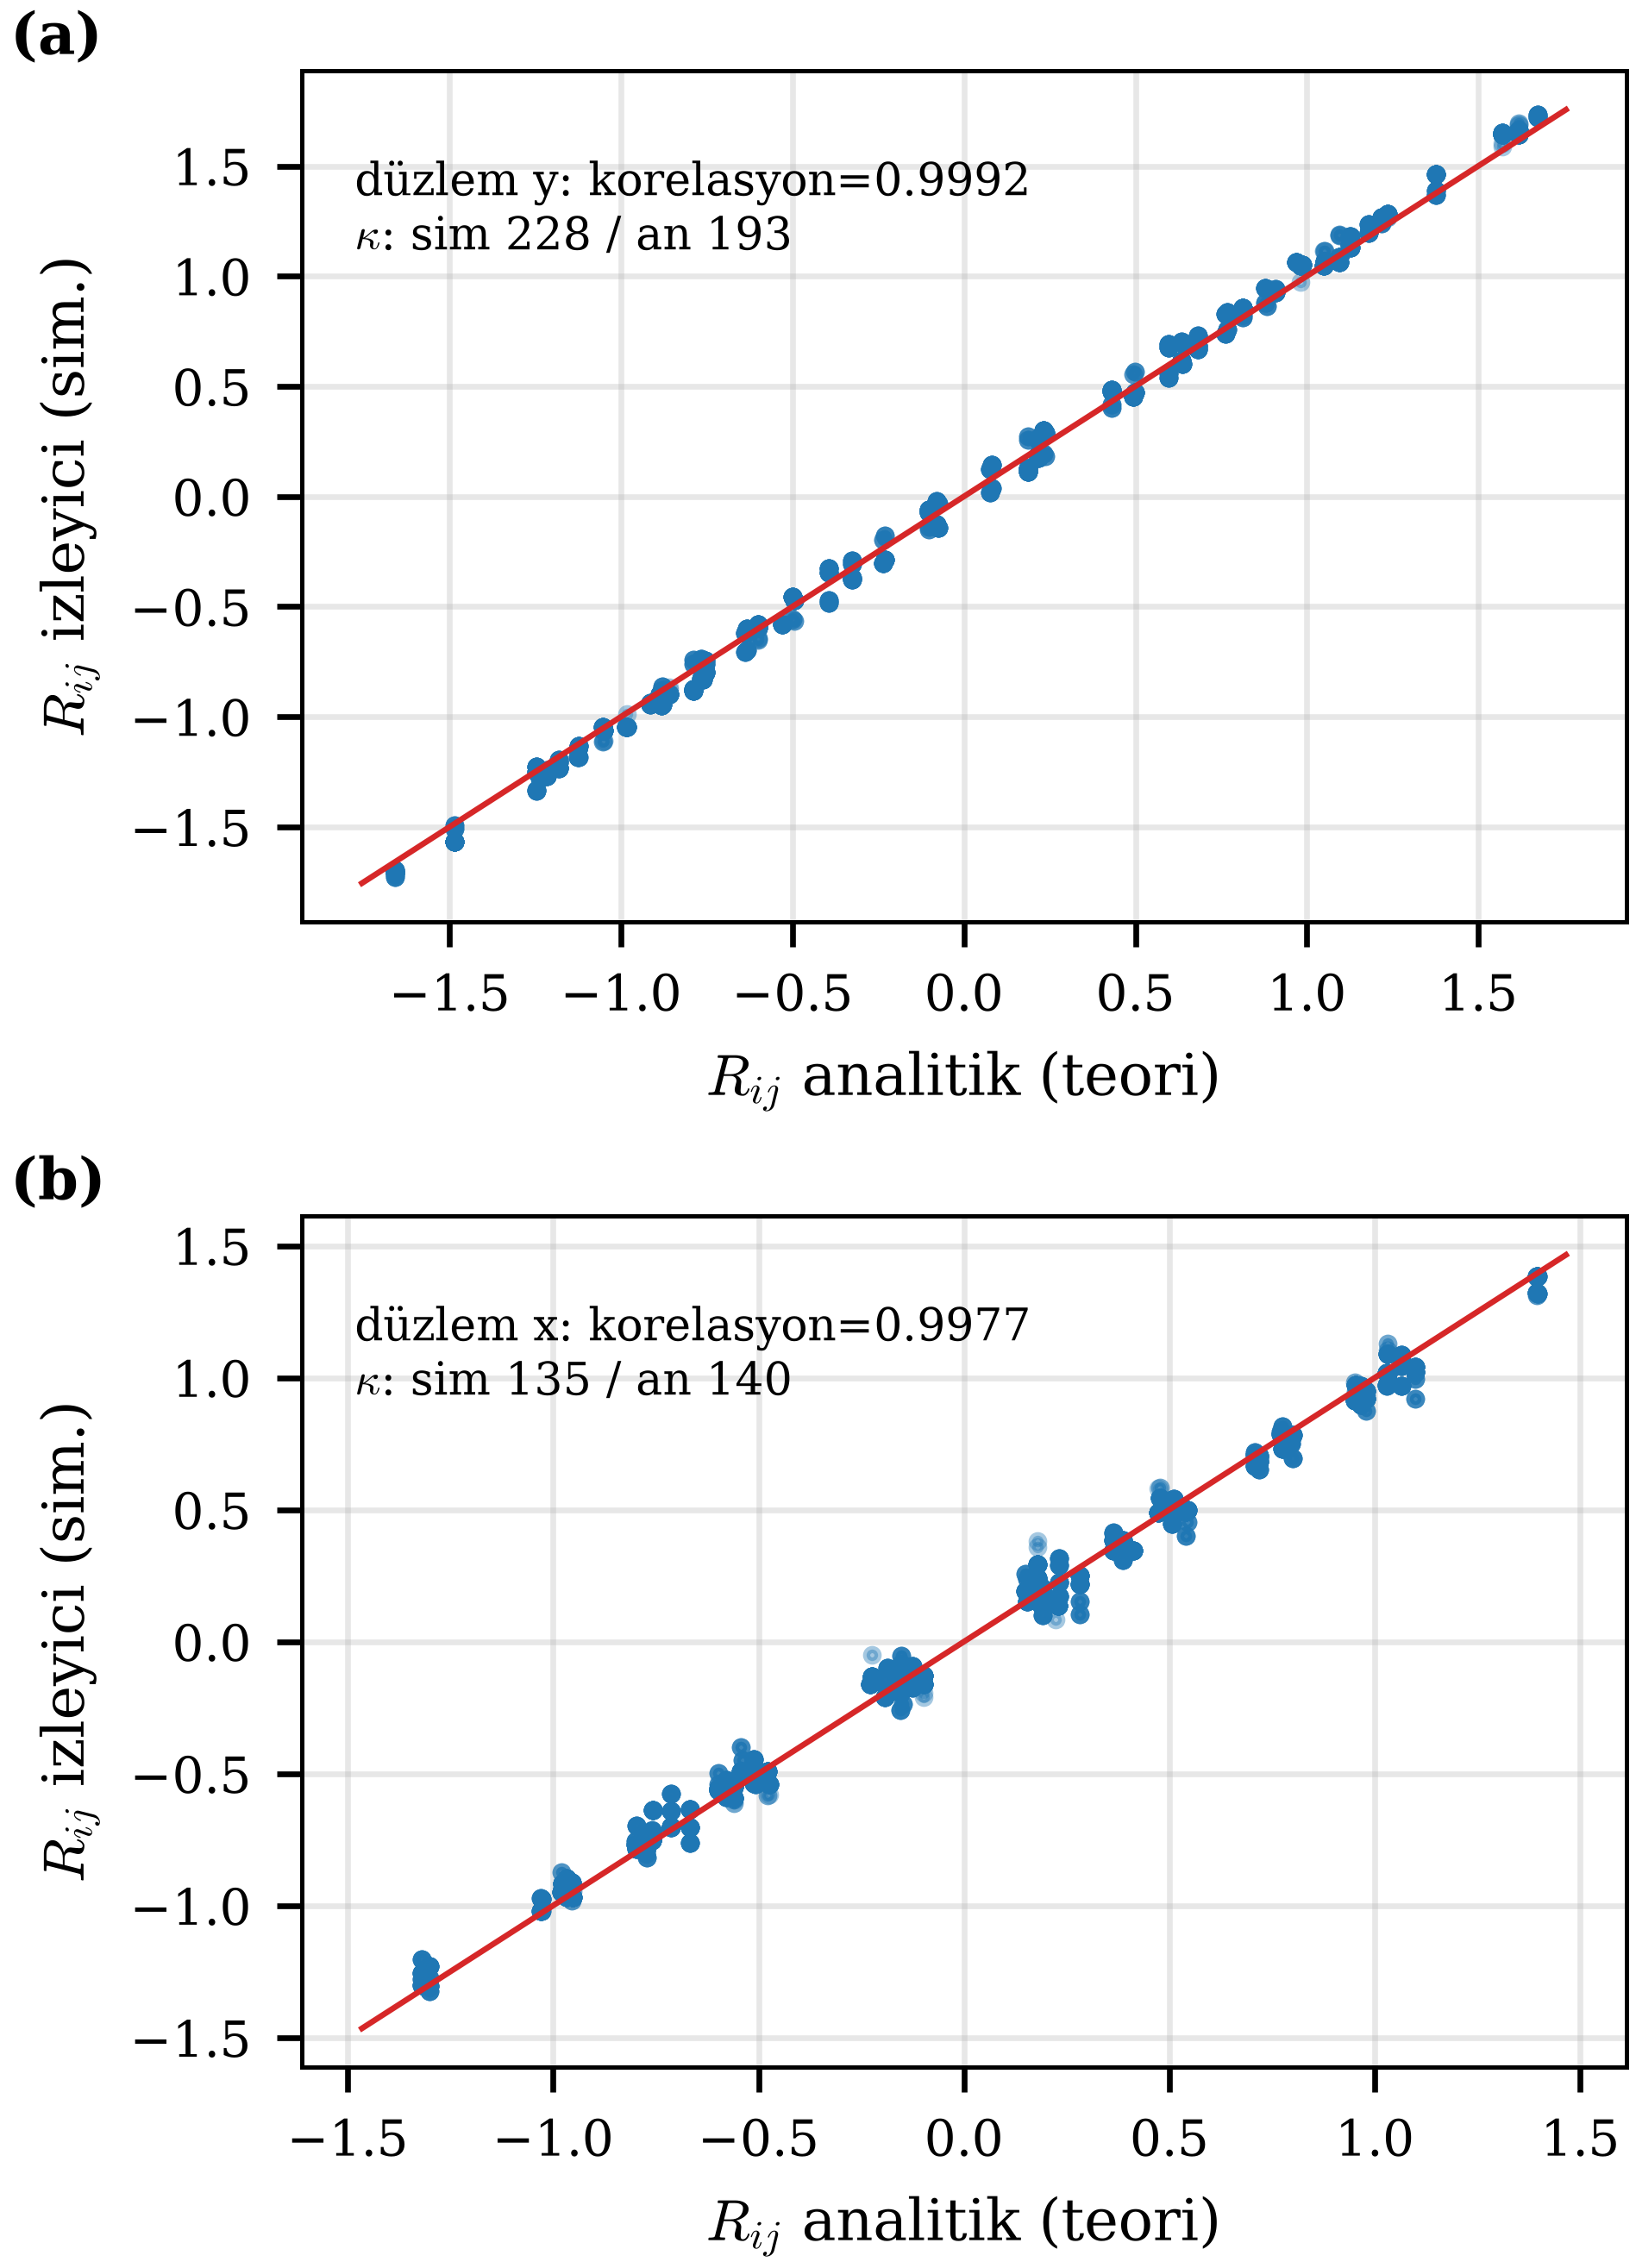
\includegraphics[width=\columnwidth]{fig7_theory_sim.png}
\caption{Analitik Courant-Snyder R (teori) ile tam parçacık izleyicisinden
(C++ GL4, \texttt{integrator.cpp}) kurulan R'nin eleman-eleman karşılaştırması;
(a) dikey, (b) yatay düzlem. Noktalar $y=x$ üzerinde: korelasyon
$0.9992/0.9977$, $\kappa$ tutarlı. Drift makalesinin analitik temelini tam
parçacık dinamiğiyle doğrular.}
\label{fig:thsim}
\end{figure}

\subsection{Aday estimatörler}
Aday yöntemler iki sınıfa ayrılır: ofseti tahmin etmeye/iptal etmeye çalışan
\textbf{mutlak rekonstrüksiyon} yaklaşımları (i--iii) ve ofseti bir nuisance
(rahatsızlık) parametresi gibi eleyip yalnız değişimi kestiren \textbf{göreli
kararlılık izlemesi} (iv).

\paragraph{(i) Mutlak tek-gradient.} $\widehat{\Delta q}=R^{-1}\mathbf{y}$.
$\kappa(R)$ küçük olduğundan gürültü iyi kontrol altındadır, ancak BPM ofseti
$R^{-1}\mathbf{b}$ olarak tahmine doğrudan sızar. Mutlak hizalama bilgisini
ofsete kurban eder.

\paragraph{(ii) İki-gradient $\Delta R^{-1}$ (ofset-iptal).}
$g_2=g_1(1+\varepsilon)$ ile iki ayrı gradient ayarında ölçüm alıp
$\widehat{\Delta q}=\Delta R^{-1}(\mathbf{y}_1-\mathbf{y}_2)$,
$\Delta R=R_1-R_2$. Ofset iptal olur, fakat $R\propto(KL)\propto g$ olduğundan
küçük $\varepsilon$ için $\Delta R\approx\varepsilon\,(g\,\partial R/\partial
g)$ olur; bu, ofset-iptal eden estimatörün \textbf{gürültü büyütmesini}
$\|\Delta R^{-1}\| = 1/\sigma_{\min}(\Delta R)\propto 1/\varepsilon$ olarak
patlatır (asıl sorun budur). Dikkat: $1/\varepsilon$ ile ölçeklenen kondisyon
sayısı $\kappa(\Delta R)$ \textbf{değil} --- o, türev matrisi
$g\,\partial R/\partial g$'nin koşulluluğu olup $\varepsilon$'dan kabaca
bağımsızdır ($\sim 10^4$, $\kappa(R)\approx 193$'ün $\sim$2 mertebe üstünde).
Pratikte ($\varepsilon\approx 0.02$) gürültü büyütmesi
$\|\Delta R^{-1}\|\sim 10^4$ mertebesine çıkar (Şekil~\ref{fig:svd},
Şekil~\ref{fig:eps}).

\paragraph{(iii) $\Delta R^{-1}$ + düzenlileştirme.} Tikhonov / TSVD.
Gürültü-bias dengesi; en iyi durumda dahi $\sim 50\,\mu$m (\S3.1).

\paragraph{(iv) Drift modu (kalibrasyon-referans) --- önerilen.} Tek gradient,
iki \emph{zaman}:
\begin{equation}
\widehat{\delta q}(t)=R^{-1}\bigl(\mathbf{y}(t)-\mathbf{y}_0\bigr).
\label{eq:drift}
\end{equation}
Sabit ofset zaman farkında iptal olur; geriye yalnızca
$\sqrt{2}\,\sigma_\eta\|R^{-1}\|$ gürültüsü kalır. Yöntem mutlak hizalamayı
değil, kalibrasyondan beri \textbf{değişimi} kestirir; mutlak referans dış
kaynaktan (LOCO/BBA) gelir (\S5).

\subsection{Ofset--gürültü dualitesi: bir önerme (destekleyici)}
Bu bölüm, aday (ii)'nin gürültü büyütmesinin algoritmik değil \textbf{yapısal}
olduğunu, dolayısıyla ``iki gradient farkıyla ofseti iptal et'' fikrinin neden
çıkmaz olduğunu gösterir. Sonuç, aşağıda açıkça tanımlanan dar bir estimatör
sınıfı için geçerli bir tekillik önermesidir (genel bir teorem iddiası
değildir).

\paragraph{Estimatör sınıfı $\mathcal{C}$.} Şu dört koşulu sağlayanlar:
(1) \emph{Lineerlik:} $\widehat{\Delta q}=A_1\mathbf{y}_1+A_2\mathbf{y}_2$;
(2) \emph{İki-ölçüm:} aynı $\Delta q$ ve aynı $\mathbf{b}$ ile
$\mathbf{y}_a=R_a\Delta q+\mathbf{b}+\eta_a$, $a\in\{1,2\}$;
(3) \emph{Ön-yargısızlık:} her $\Delta q$ için
$\mathbb{E}[\widehat{\Delta q}]=\Delta q$;
(4) \emph{Tam ofset iptali:} her sabit $\mathbf{b}$ tahmine sızmaz.

\paragraph{İddia.} $\mathcal{C}$ içinde tek çözüm $A_1=\Delta R^{-1}$,
$A_2=-\Delta R^{-1}$'dir.

\paragraph{Türetiş.} Koşul (3): $A_1R_1+A_2R_2=I$. Koşul (4):
$A_1+A_2=0\Rightarrow A_2=-A_1$. Birleştirince
$A_1(R_1-R_2)=I\Rightarrow A_1=\Delta R^{-1}$. $\blacksquare$

\paragraph{Sonuç.} $\mathcal{C}$ içindeki tek çözümün gürültü büyütmesi
$\|\Delta R^{-1}\|$'dir; $\Delta R\approx\varepsilon R$ ile yaklaşık
$\|R^{-1}\|/\varepsilon$. Bu, $\varepsilon\to 0$ sınırında patlar (\S3.2'de SVD
spektrumuyla doğrulanır). Önemli nokta: \textbf{drift modu (iv) $\mathcal{C}$
dışındadır} --- iki ölçüm aynı anda değil iki farklı \emph{zamanda} alınır ve
estimatör $\Delta q$'yu değil $\delta q(t)=\Delta q(t)-\Delta q_0$'ı kestirir.
Ofset zaman farkıyla iptal olur, kondisyon sayısı $\kappa(R)\approx 193$
kalır. $\mathcal{C}$ dışındaki diğer yaklaşımlar (Tikhonov/TSVD, Bayesçi,
Kalman, çok-epoch) bu sınıra uymak zorunda değildir.

% ============================================================
\section{Sayısal Deneyler}
Tüm testler ortak bir altyapıda koşuldu (Ek~A): semplektik izleyici, gerçekçi
BPM gürültü ve ofset modeli, opsiyonel quad/dipol tilt'leri. Hızlandırıcı
parametreleri \texttt{params.json}, test parametreleri
\texttt{test\_params.json} içindedir.

\subsection{Test 1 --- Düzenlileştirme ham $\Delta R^{-1}$'i kurtarır mı?}
BPM ofseti \textbf{yok}; bu test ideal şartta gürültü tabanını ölçer. Aynı
veride dört estimatör (Tablo~\ref{tab:t1}). \textbf{Uyarı:} Direct $R^{-1}$
operasyonel bir rakip değildir; ofset sıfır varsayımına dayanır ve gerçek
halkada ($\mathbf{b}\neq 0$) 200+\,$\mu$m'e tırmanır (Test~4). Tabloda yalnızca
gürültü tabanı referansı olarak yer alır. Düzenlileştirme ham (ii)'yi
$\sim 35\times$ iyileştirir ama korelasyon 0.998'den 0.35'e düşer (RMS azalır,
biçim bozulur) ve hâlâ 10\,$\mu$m hedefinin çok üstündedir.

\begin{table}[tb]
\centering\small
\caption{Test 1: ofsetsiz ideal şartta dört estimatör.}
\label{tab:t1}
\begin{tabular}{@{}lrrl@{}}
\toprule
Estimatör & $y$-RMS & $y$-kor & Yorum \\
          & [$\mu$m] &        &       \\
\midrule
Direct $R^{-1}$        & 3.5  & 0.998 & gürültü tabanı \\
Ham $\Delta R^{-1}$    & 1865 & 0.085 & \S2.4 sınırı \\
Tikhonov (L-curve)     & 53   & 0.348 & bias--varyans \\
TSVD ($k{=}3$, oracle) & 52   & 0.383 & oracle üst-sınır \\
\bottomrule
\end{tabular}
\end{table}

\subsection{Test 2 --- Uzaysal transfer fonksiyonu ve SVD spektrumu}
Saf sinüsoidal patern girişine ($\Delta q_j=A\cos(2\pi kj/N)$) estimatör mod
transferi: Tikhonov/TSVD yüksek-$k$ modlarını ($k\gtrsim 18$) tamamen söndürür;
48 modun yalnızca 3--5'i kurtarılır. SVD spektrumu yan yana çizildiğinde
$\Delta R\approx\varepsilon R$ bulk ölçeklemesi doğrulanır
(Şekil~\ref{fig:svd}): $\Delta R$'nin büyük singüler değerleri $R$'ninkilerin
yaklaşık $\varepsilon$ katıdır; en küçük modlar ise bu ölçeklemenin altına
çöker, $\Delta R$ her durumda $R$'den $\sim$2 mertebe kötü koşulludur.

$\varepsilon$ taraması (Şekil~\ref{fig:eps}) asıl ölçeklemeyi netleştirir:
ofset-iptal eden estimatörün gürültü büyütmesi
$\|\Delta R^{-1}\|=1/\sigma_{\min}(\Delta R)$ tüm
$\varepsilon\in[0.005,0.10]$ aralığında temiz biçimde $\propto 1/\varepsilon$
patlarken, kondisyon sayısı $\kappa(\Delta R)$ kabaca sabit ($\sim 10^4$)
kalır. Yani $\varepsilon\to 0$ sınırında yöntemi kullanılamaz kılan $\kappa$
değil, $\|\Delta R^{-1}\|$'dir --- bu, \S2.4'teki alt-sınır önermesinin
($\|\Delta R^{-1}\|\sim\|R^{-1}\|/\varepsilon$) doğrudan sayısal
doğrulamasıdır.

\begin{figure}[tb]
\centering
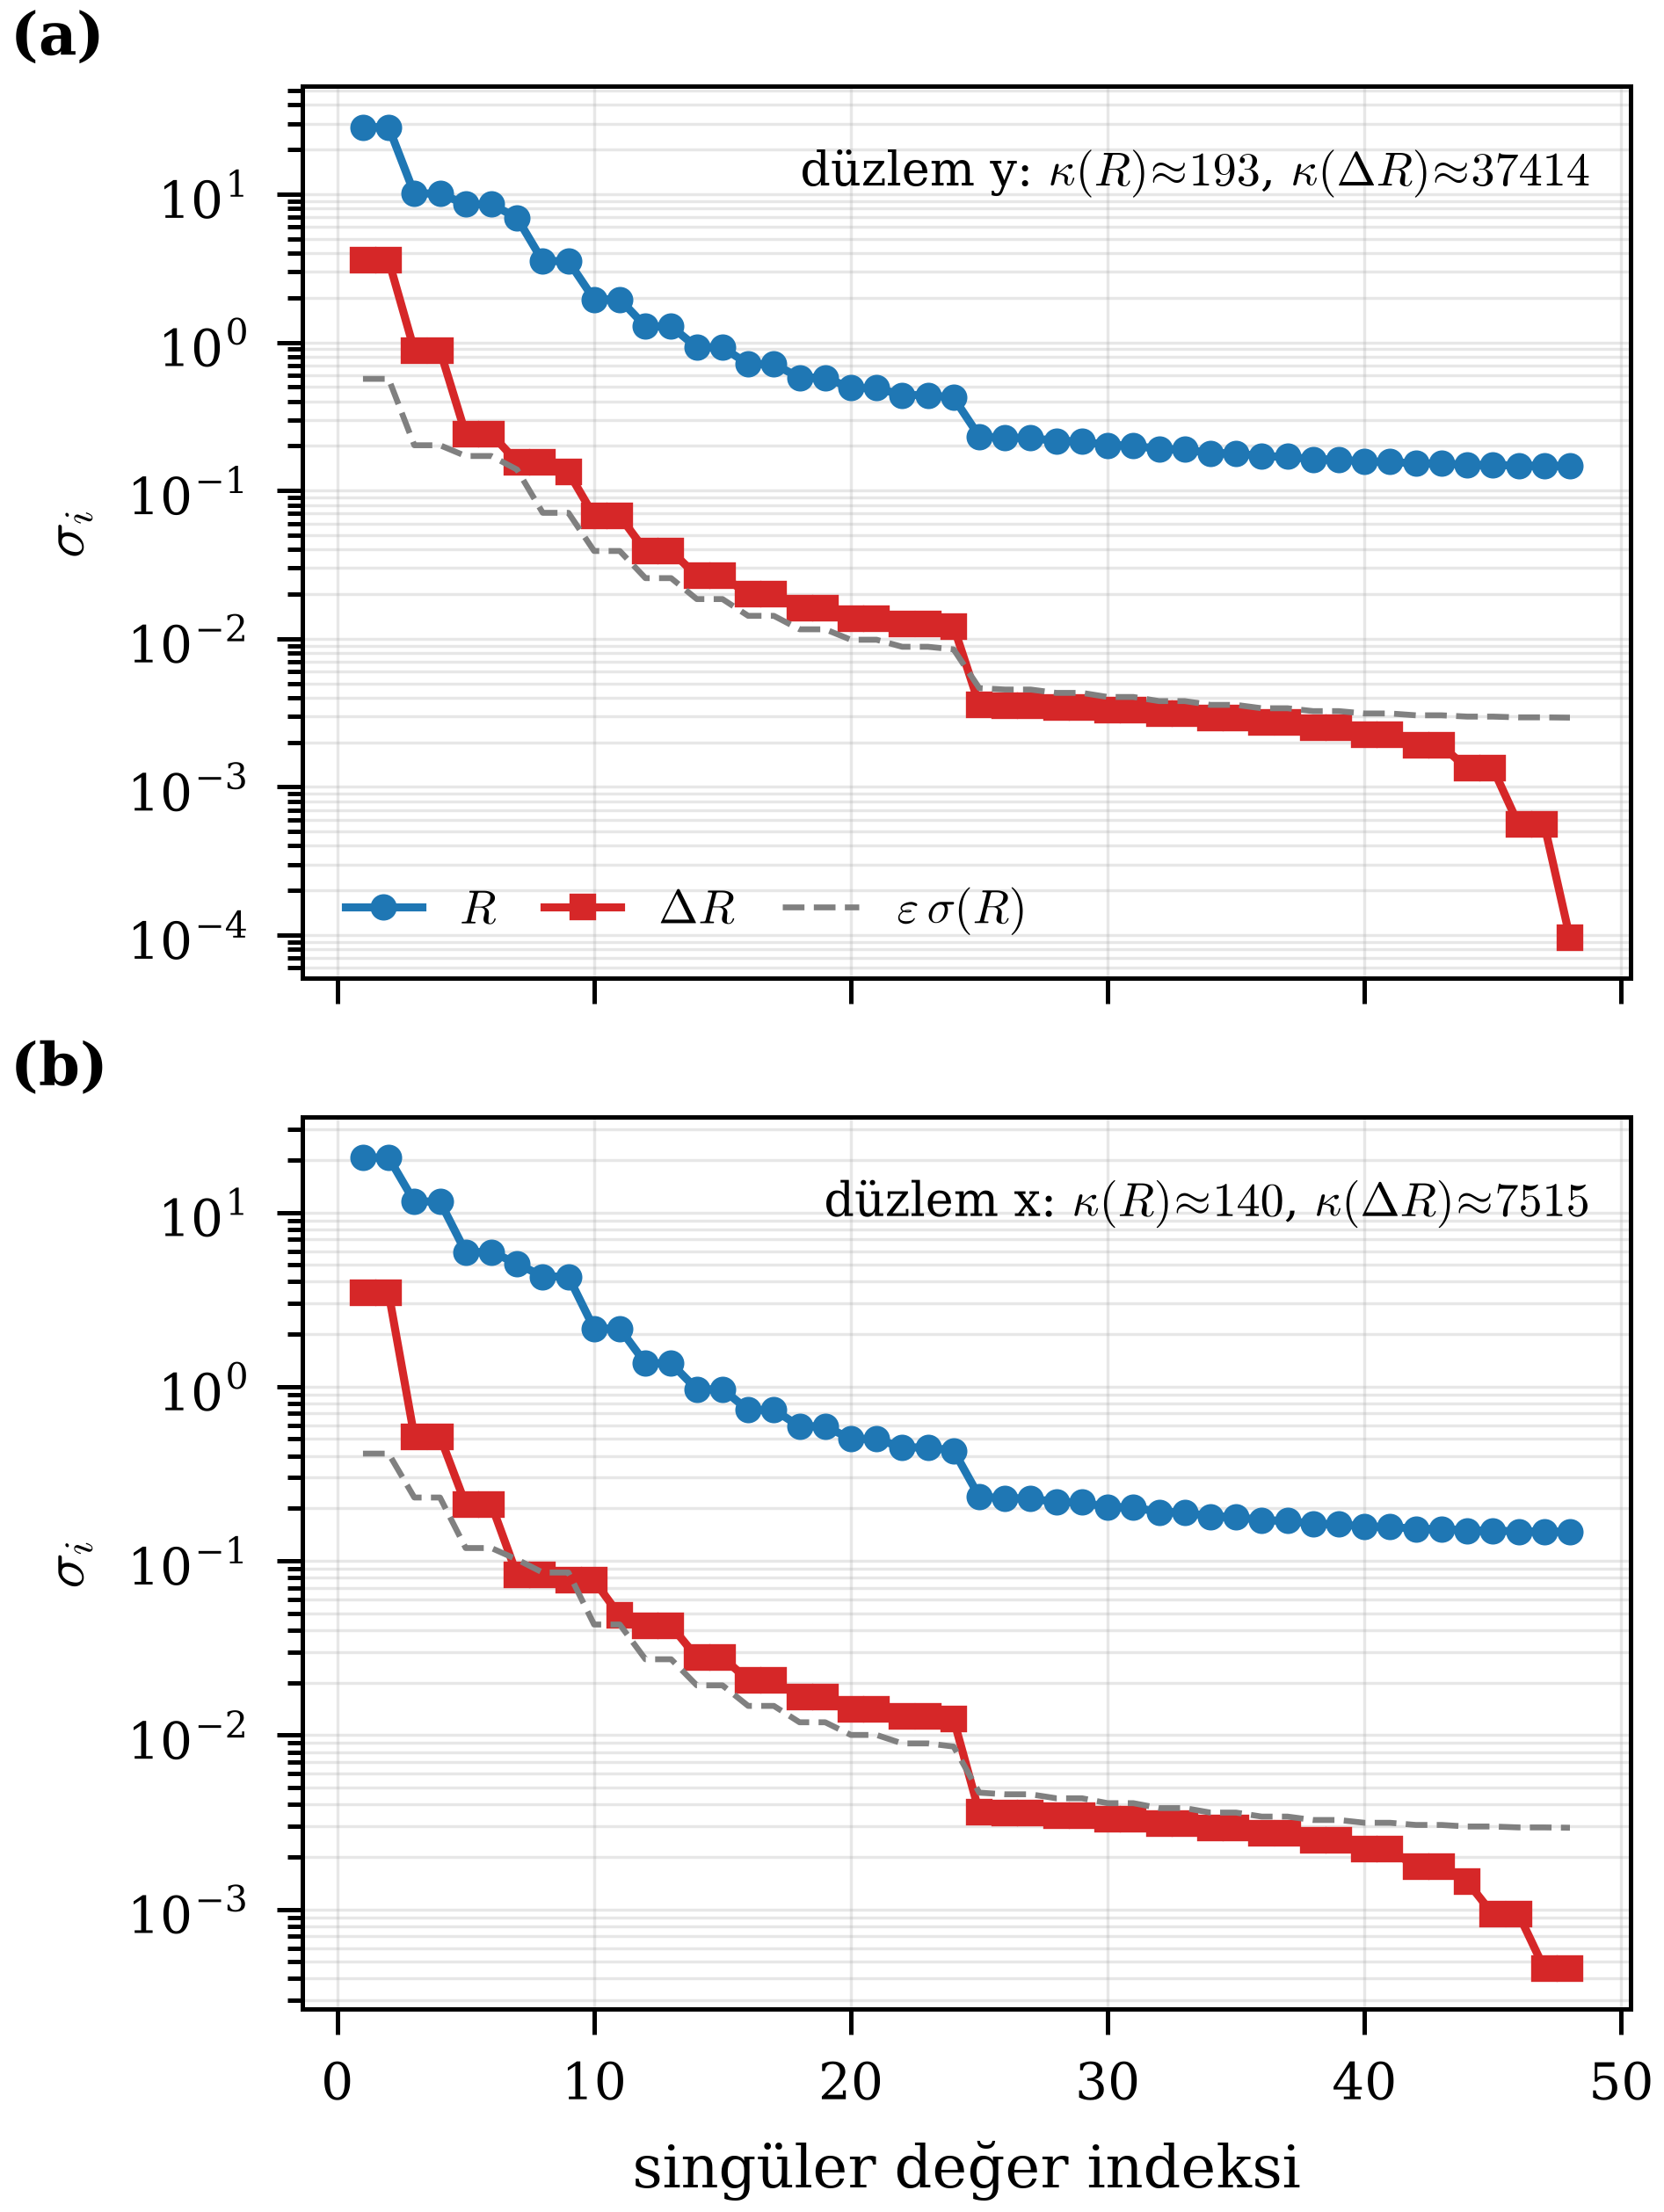
\includegraphics[width=\columnwidth]{fig1_svd_spektrum.png}
\caption{Tepki matrisi $R$ ve iki-gradient farkı
$\Delta R=R(g_1)-R(g_1(1+\varepsilon))$ ($\varepsilon=0.02$) için
singüler-değer spektrumları; (a) dikey, (b) yatay düzlem. Kesikli gri çizgi
$\varepsilon\,\sigma(R)$ beklenen bulk ölçeklemesidir. $\Delta R$'nin büyük
singüler değerleri bu çizgiyi izler; en küçük modlar daha da çöker. $R$ iyi
koşulludur ($\kappa\approx 193/140$), $\Delta R$ ise $\sim$2 mertebe kötüdür.}
\label{fig:svd}
\end{figure}

\begin{figure}[tb]
\centering
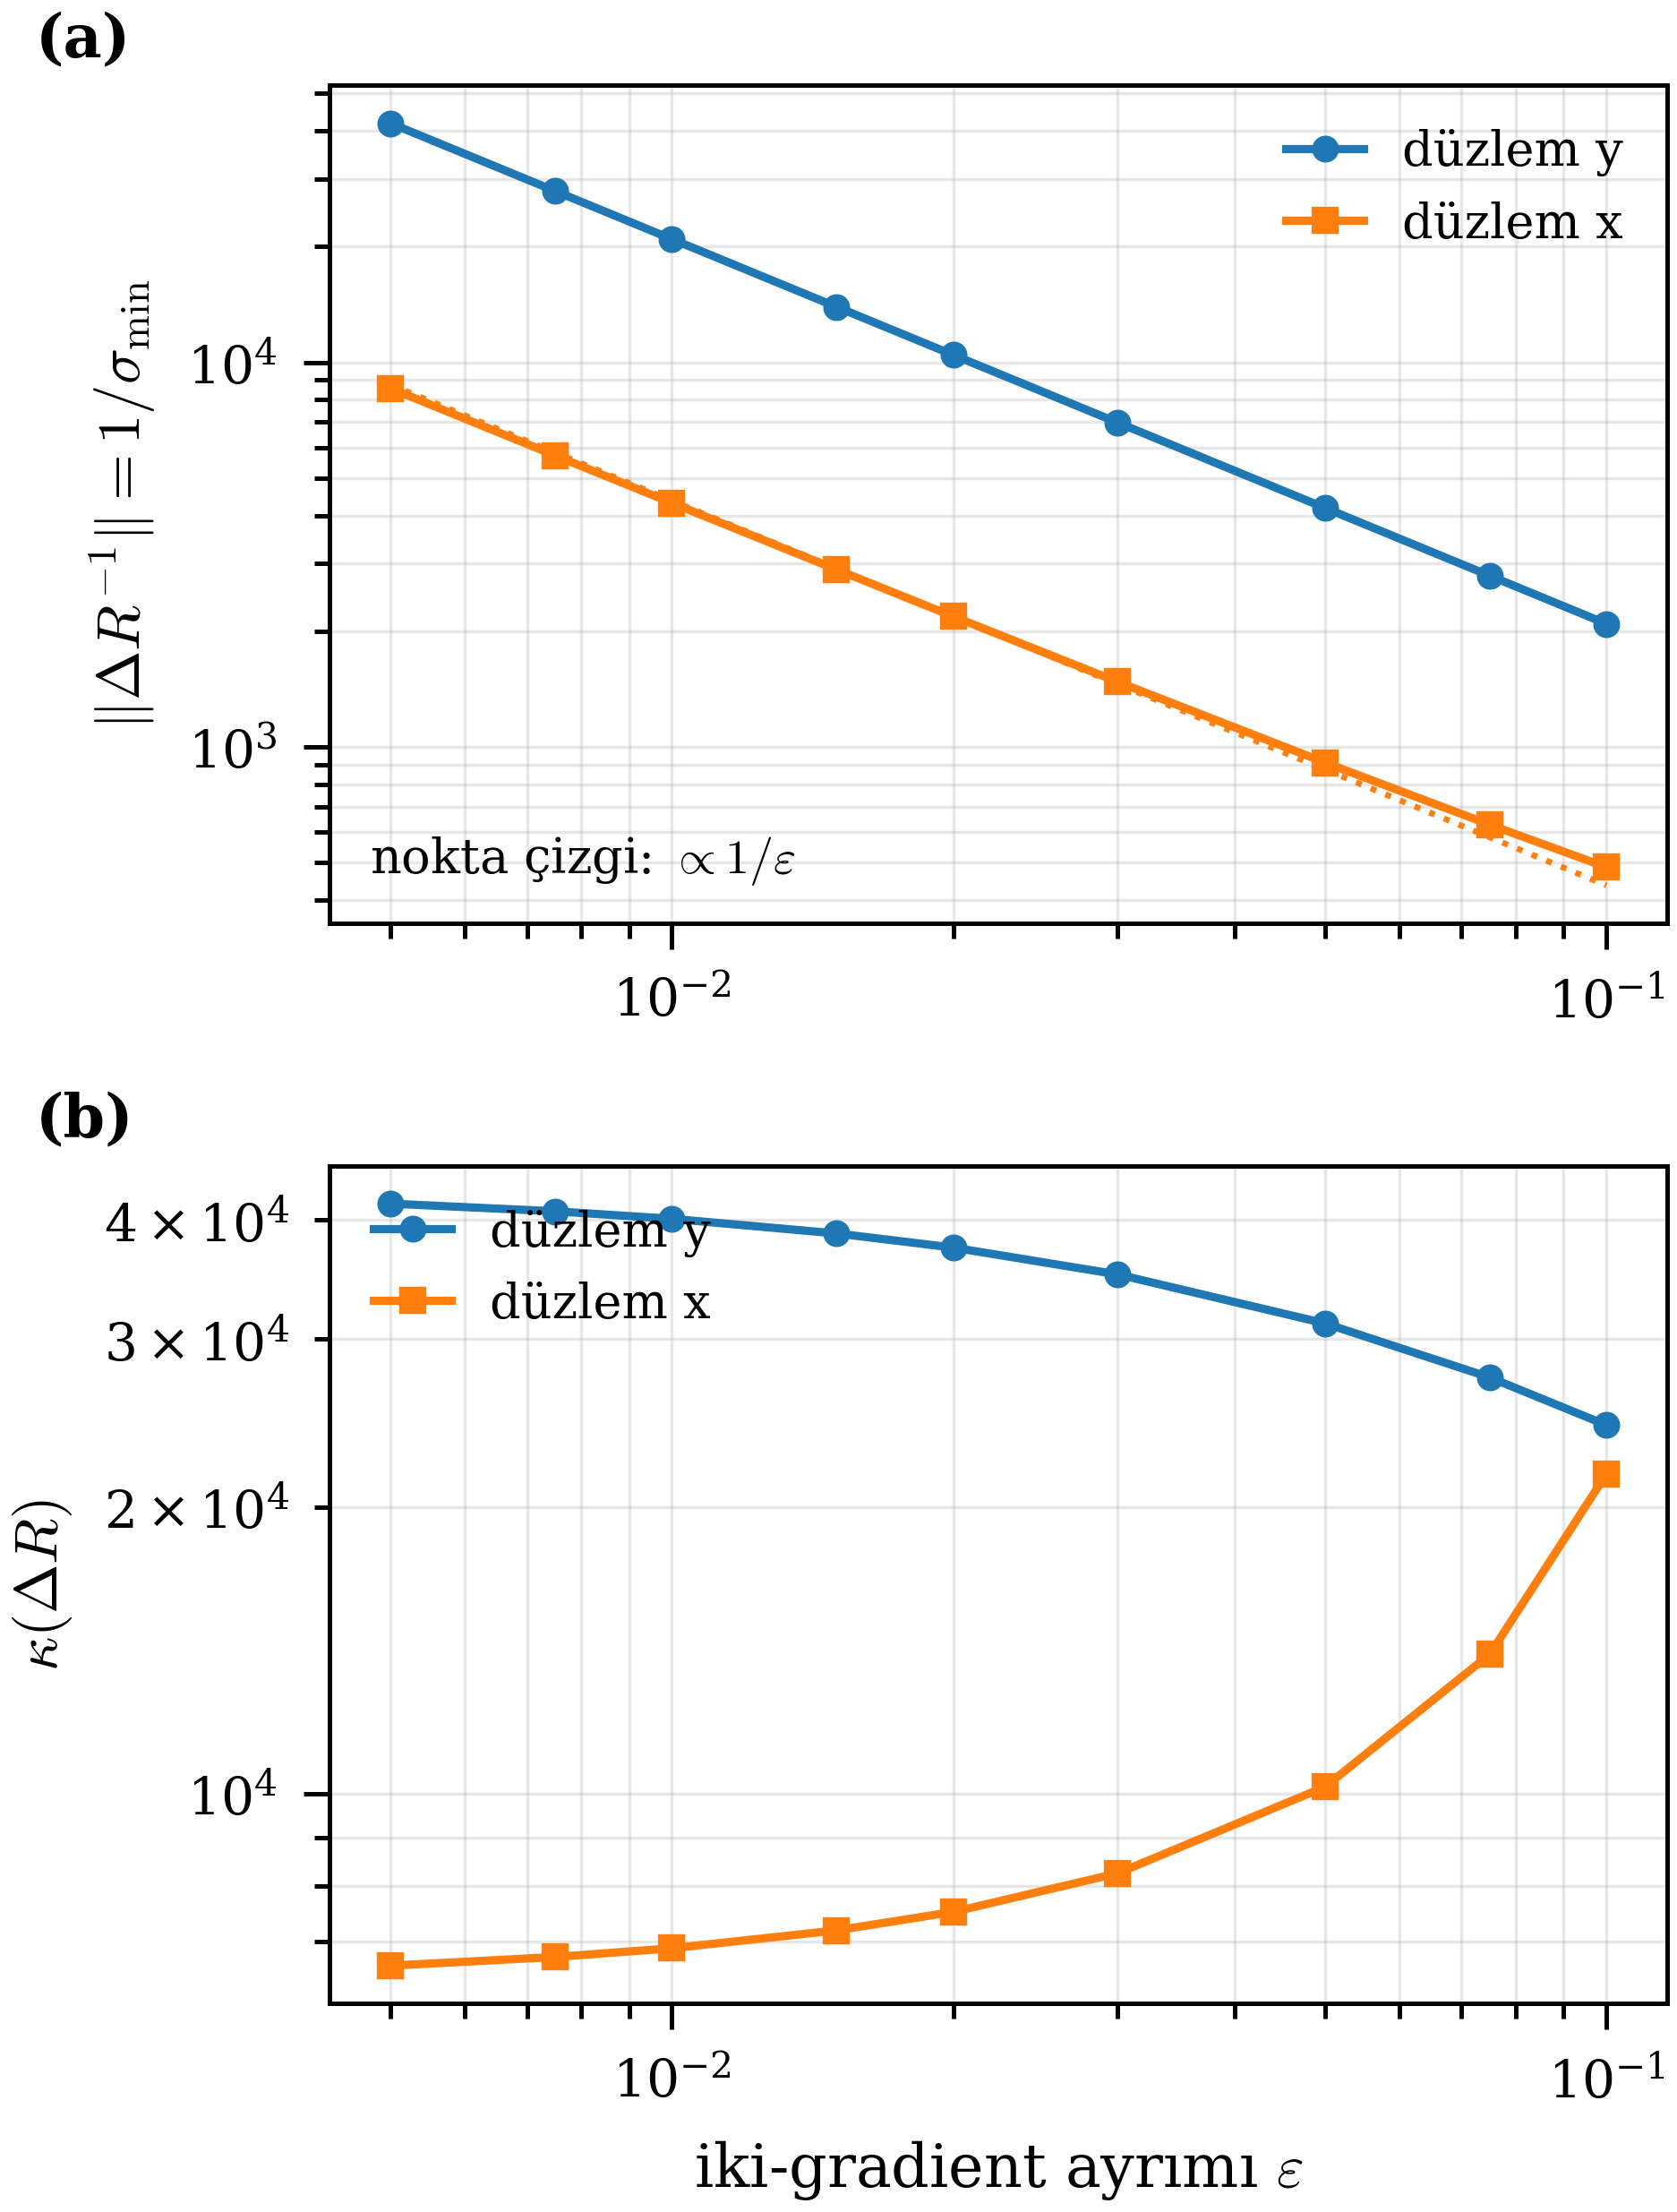
\includegraphics[width=\columnwidth]{fig6_epsilon_sweep.png}
\caption{$\varepsilon$ taraması: (a) ofset-iptal eden estimatörün gürültü
büyütmesi $\|\Delta R^{-1}\|=1/\sigma_{\min}(\Delta R)$, noktalı
$1/\varepsilon$ referansıyla --- temiz $1/\varepsilon$ ölçeklemesi;
(b) kondisyon sayısı $\kappa(\Delta R)$, $\varepsilon$'dan kabaca bağımsız
($\sim 10^4$). $\varepsilon\to0$'da yöntemi bozan $\kappa$ değil
$\|\Delta R^{-1}\|$'dir.}
\label{fig:eps}
\end{figure}

\subsection{Test 3 --- Yatay model ters-suç kontrolü}
$K_{x,\text{arc}}$ kalibrasyonu simülasyondan alınır (klasik ters-suç).
$K_{x,\text{arc}}(1+\delta)$, $\delta\in[-10\%,+10\%]$ taramasında yatay RMS
3.48--4.01\,$\mu$m (0.5\,$\mu$m değişim); dikey sabit (Maxwell). Gerçek halkada
LOCO'nun sağladığı $<1\%$ doğrulukta yöntem \textbf{operasyonel olarak
ters-suçtan bağımsız}.

\subsection{Test 4 --- Drift modunun kalibrasyon-referansla gösterimi}
\textbf{Senaryo.} $t=0$: 100\,$\mu$m RMS hizalama + 50\,$\mu$m RMS BPM ofseti
kaydedilir. $t=1..10$: hizalama 10\,$\mu$m RMS yavaşça kayar, ofset sabit.
50\,$\mu$m RMS ofset yöntemi etkilemez; geriye yalnızca gürültü-kaynaklı taban
kalır (Şekil~\ref{fig:drift}, Tablo~\ref{tab:t4}).

\begin{table}[tb]
\centering\small
\caption{Test 4: mutlak vs drift modu (RMS hata).}
\label{tab:t4}
\begin{tabular}{@{}lcc@{}}
\toprule
Yöntem & Düzlem $y$ & Düzlem $x$ \\
\midrule
Mutlak $R^{-1}\mathbf{y}(t)$ & $\sim$197\,$\mu$m & $\sim$185\,$\mu$m \\
\textbf{Drift $R^{-1}(\mathbf{y}-\mathbf{y}_0)$}
                             & \textbf{6.6\,$\mu$m} & \textbf{6.5\,$\mu$m} \\
İyileşme                     & $29\times$ & $28\times$ \\
\bottomrule
\end{tabular}
\end{table}

\begin{figure}[tb]
\centering
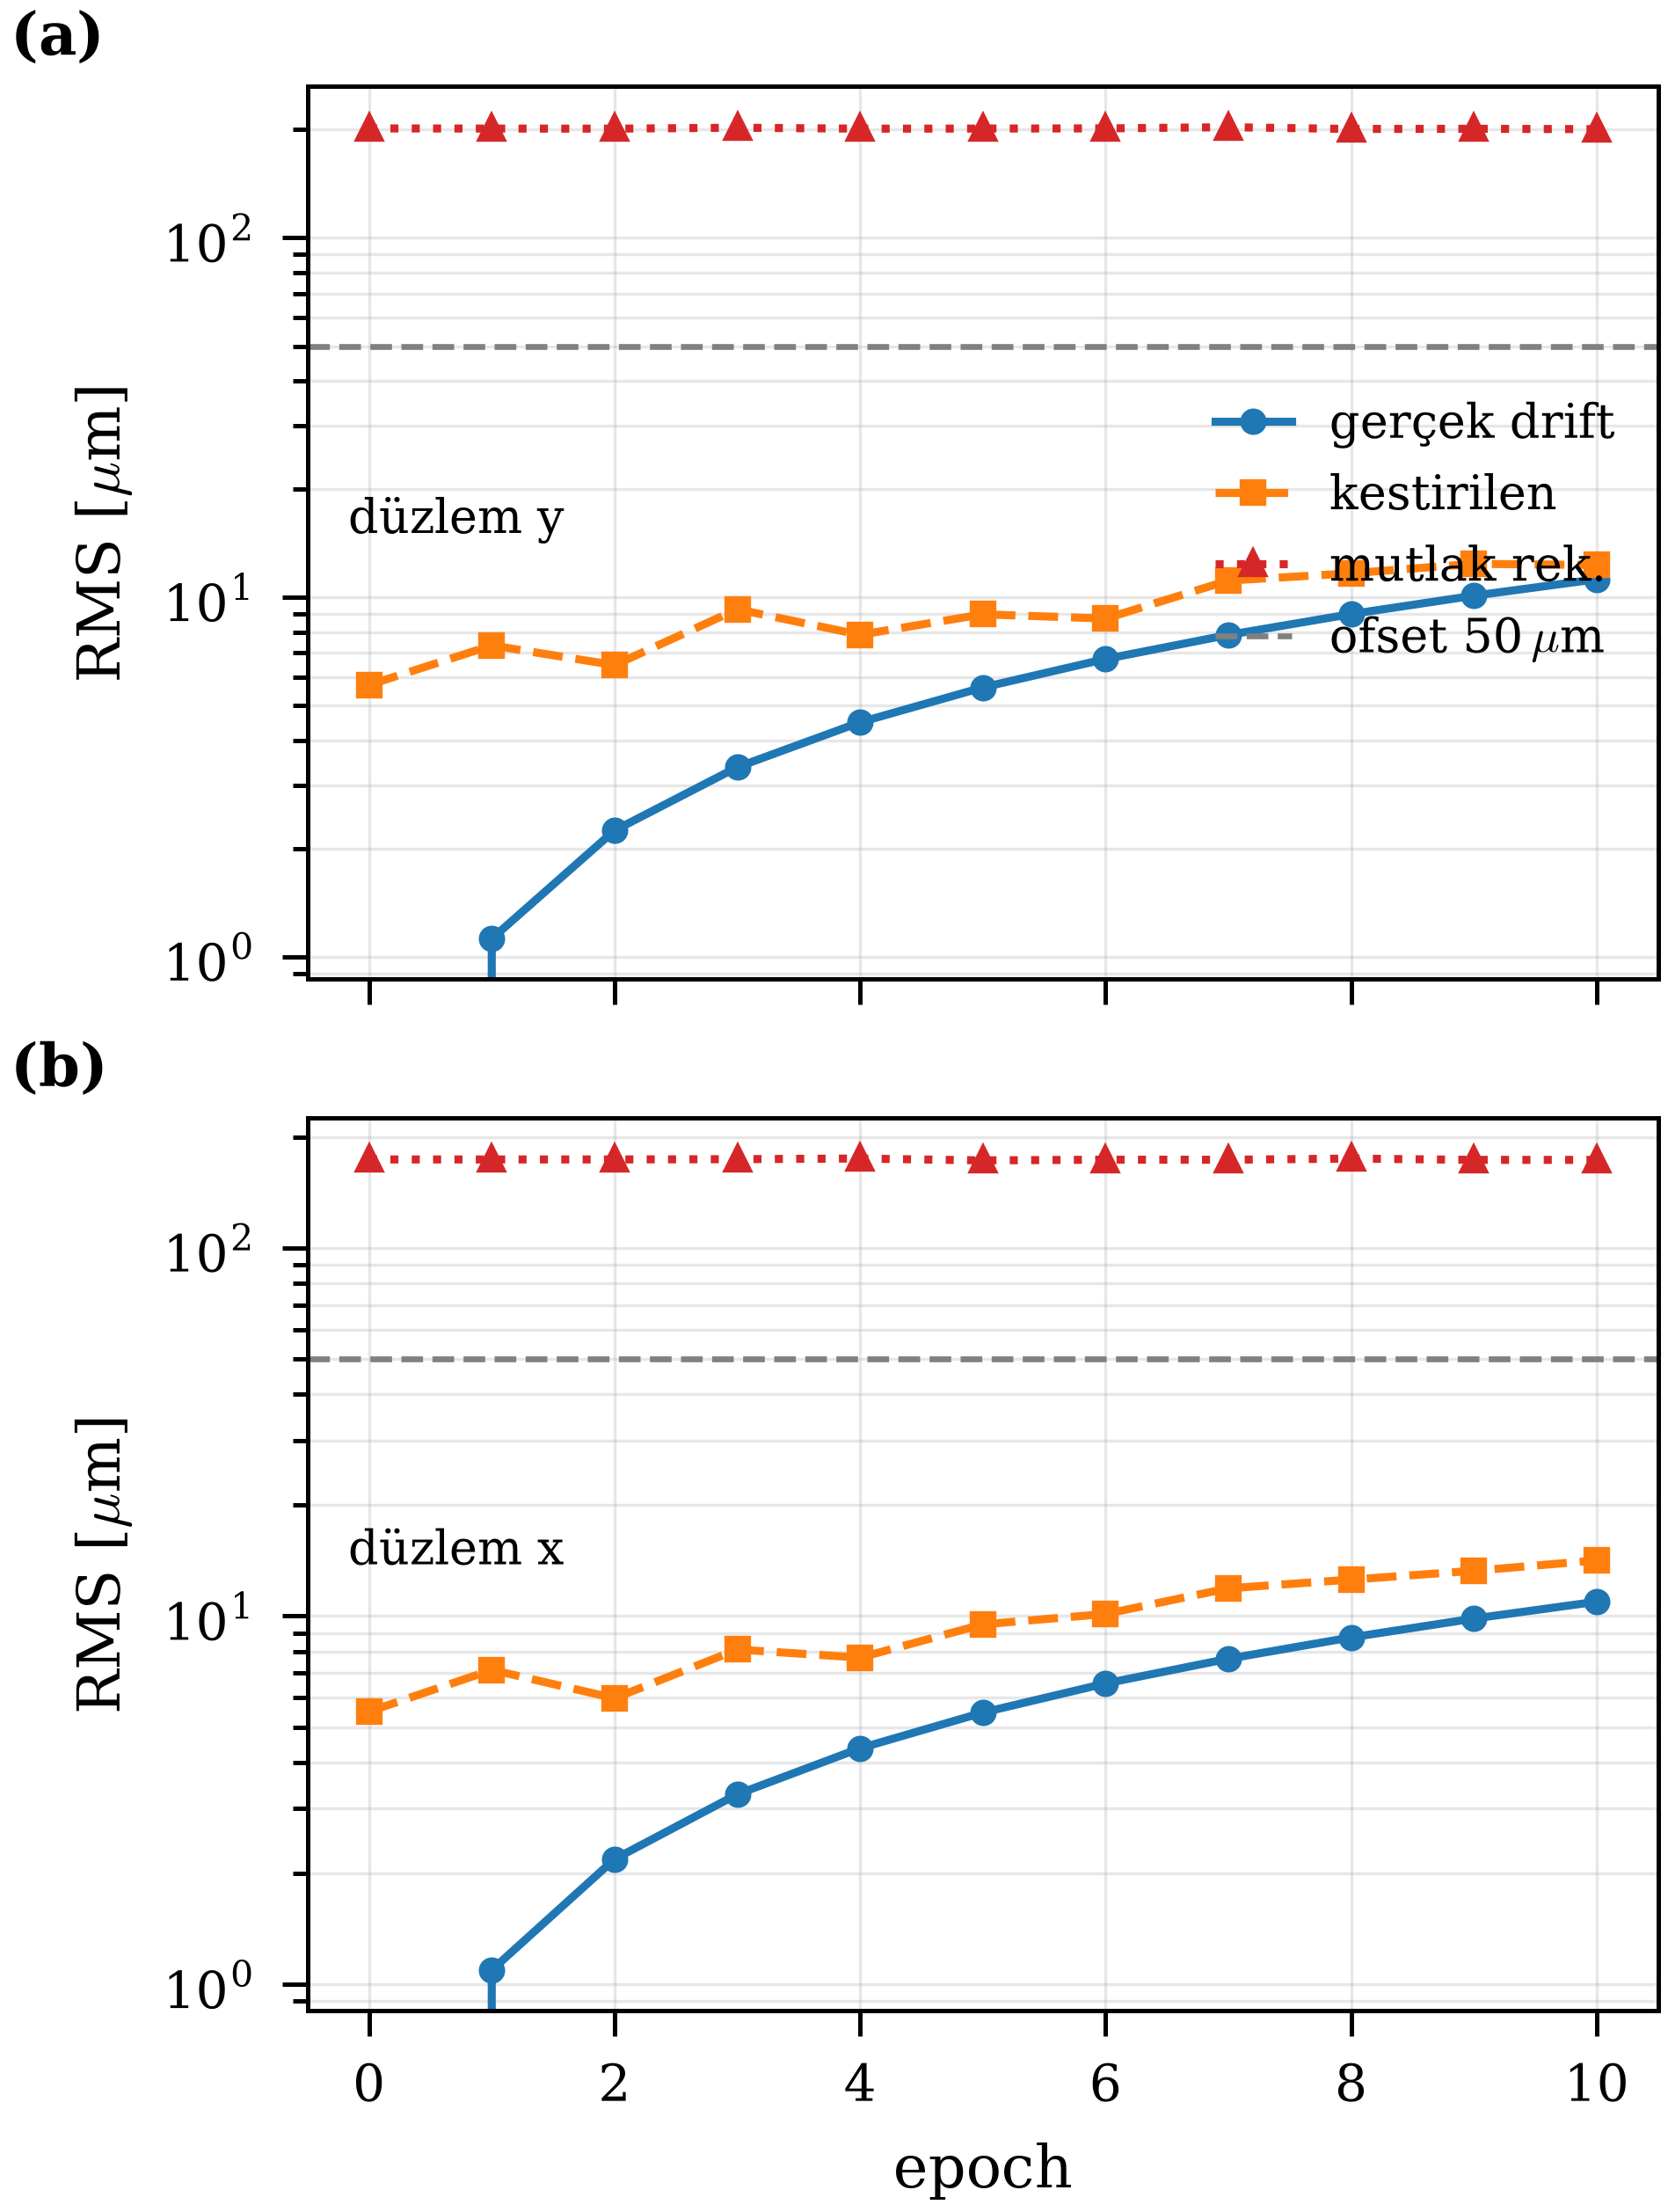
\includegraphics[width=\columnwidth]{fig2_drift_izleme.png}
\caption{Test 4 kalibrasyon-referans drift izleme, (a) dikey, (b) yatay
düzlem. Gerçek drift, kestirilen drift ve naif mutlak rekonstrüksiyon hatası
epoch'a karşı (log ölçek). 50\,$\mu$m BPM ofseti mutlak rekonstrüksiyonu
$\sim$200\,$\mu$m'de boğarken drift modu 6--7\,$\mu$m RMS'te izler.}
\label{fig:drift}
\end{figure}

\subsection{Test 5 --- BPM ofseti zamanla kayarsa?}
Drift modu $\mathbf{b}(t)\approx\mathbf{b}_0$ varsayar; ofset kayma hızı
$\dot{\mathbf{b}}$ arttıkça kestirime $R^{-1}\dot{\mathbf{b}}\,\Delta t$ olarak
sızar. Simülasyonda drift modu ile per-epoch iki-gradient + 30-epoch ortalama
karşılaştırıldığında, drift modunun üstünlüğünü kaybettiği geçiş
$\sim 2\,\mu$m/epoch ofset kayma hızındadır. Bu eşiğin gerçek bir pEDM BPM
sisteminde sağlanıp sağlanmadığı \textbf{deneysel olarak doğrulanması gereken
bir gerekliliktir} (\S6); burada bir donanım iddiası yapılmamakta, yalnızca
yöntemin geçerli kaldığı kayma-hızı bütçesi nicelenmektedir.

\subsection{Test 6 --- Üç yöntemin adil karşılaştırması}
Aynı veri, aynı bütçe (50\,$\mu$m ofset, 1\,$\mu$m gürültü, 10\,$\mu$m drift,
0.2\,mrad tilt'ler); Tablo~\ref{tab:t6}. Her iki $\Delta R$ inşası da
$\kappa\sim 10^4$ mertebesinde kötü koşulludur (düzleme bağlı
$\sim 7\times10^3$--$4\times10^4$; bkz.\ Şekil~\ref{fig:svd}). Sayısal $R$,
$\Delta R$ yaklaşımını kurtarmaz --- $\kappa(\Delta R)$ matrisin nasıl inşa
edildiğine değil $\varepsilon$ ve örgü fiziğine bağlıdır. Drift modu yapısal
olarak farklı bir problem (mutlak değil, değişim) çözdüğü için bu sınırın
dışındadır.

Tablodaki $x$ ve $y$ sütunları \textbf{bağımsızdır}: bu çalışmadaki lineer model
yatay ve dikey düzlemleri ayrık ele alır (skew kuplajı = kuadrupol dönmesi
sıfır), dolayısıyla bir $x\!-\!y$ çapraz (kuplaj) terimi yoktur; her düzlem kendi
$48\times48$ sistemidir. (Sahte EDM'i süren $dx\cdot dy$ kuplajı bu lineer
yörünge modelinde değil, ikinci-derece bir spin etkisidir --- bkz.\ \S4.4.)

\paragraph{Peki gerçek quad tilt bu varsayımı kırar mı?} Kuadrupol dönmesi
(tilt) gerçek bir skew bileşeni yaratır ve $dx\to$ dikey, $dy\to$ yatay yörünge
çapraz terimlerini açar. Bunu doğrudan test ettik: rastgele quad tilt'lerle
\textbf{kuplajlı} tam tepki matrisini (dört blok $R_{yy},R_{yx},R_{xy},R_{xx}$)
izleyiciden kurup, düzlem-ayrık monitörle ($R_{yy}^{-1},R_{xx}^{-1}$) drift
kurtarımı yaptık (Tablo~\ref{tab:tilt}). Gerçekçi 0.2\,mrad tilt'te çapraz kuplaj
diyagonal tepkinin yalnız \%0.33'ü; drift takip hatası \textbf{değişmez}
($6.27\,\mu$m). 1\,mrad'a kadar (kuplaj \%1.1) hata yine sabit. Çapraz kuplaj,
drift modunun ölçtüğü \emph{değişime} $\sim$(kuplaj)$\times$(drift)
$\approx 0.1\,\mu$m katkı verir --- 6\,$\mu$m tabanının çok altında.
\textbf{Düzlem-ayrık model gerçekçi quad tilt altında geçerlidir.}

\begin{table}[tb]
\centering\small
\caption{Quad tilt kaynaklı $x\!-\!y$ kuplajı ve düzlem-ayrık drift kurtarımına
etkisi (izleyiciden kuplajlı $R$; 15-tohum medyanı).
\texttt{drift\_quadtilt\_sim.py}}
\label{tab:tilt}
\begin{tabular}{@{}lccc@{}}
\toprule
Quad tilt & $\|R_{yx}\|/\|R_{xx}\|$ & $y$-takip [$\mu$m] & $x$-takip [$\mu$m] \\
\midrule
0          & \%0.00 & 6.27 & 5.95 \\
\textbf{0.2\,mrad} & \textbf{\%0.33} & \textbf{6.27} & \textbf{5.95} \\
1\,mrad    & \%1.08 & 6.26 & 5.95 \\
\bottomrule
\end{tabular}
\end{table}

\begin{table*}[tb]
\centering
\caption{Test 6: aynı senaryoda üç estimatörün yan yana karşılaştırması.}
\label{tab:t6}
\begin{tabular}{@{}lrrrr@{}}
\toprule
Estimatör & $y$-RMS [$\mu$m] & $y$-kor & $x$-RMS [$\mu$m] & $x$-kor \\
\midrule
A: analitik $\Delta R$        & 3282 & $-0.02$ & 3756 & $0.09$ \\
\textbf{B: drift modu}        & \textbf{6.25} & \textbf{0.85} & \textbf{7.18} & \textbf{0.85} \\
C: sayısal $\Delta R$         & 980  & $-0.02$ & 1357 & $-0.11$ \\
\bottomrule
\end{tabular}
\end{table*}

\subsection{Test 8 --- Örgü modeli hatası altında $\beta$-beating sağlamlığı}
Drift modu $R^{-1}$'in doğruluğuna bağlıdır. Gerçek halkada LOCO + BBA sonrası
$\sim$\%1--5 $\beta$-beating ve faz hatası kalır. Nominal model
$R_\text{nom}$ ile gerçek makine $R_\text{true}$ ($\beta,\phi$'de
$\varepsilon_\beta$ bozunumu) arasında kasıtlı uyumsuzluk; veri
$R_\text{true}$, kestirim $R_\text{nom}^{-1}$ ile (15 tohum medyanı,
Tablo~\ref{tab:t8}). LOCO sonrası tipik $\sim$\%1 $\beta$-beating'de taban
yalnızca 0.1\,$\mu$m artar (5.98$\to$6.08\,$\mu$m); hedefe 3.9\,$\mu$m marj
kalır. Yöntem, standart-kalite LOCO'su olan bir hızlandırıcıda operasyonel
olarak kullanılabilir (Şekil~\ref{fig:beta}).

\paragraph{İzleyici doğrulaması --- ve focal length hatası nereye düşüyor.}
Yukarıdaki tarama $\beta$-beating'i analitik olarak ($\beta,\phi$ doğrudan
bozularak), yani \emph{belirtiyi} modelliyordu. Bunu $\beta$-beating'in fiziksel
\emph{kaynağıyla} tekrarladık: \textbf{kuadrupol odak-uzaklığı (focal length)
hataları.} Bir kuadrupolün odak uzaklığı $1/f=(G/B\rho)\,L$ gradyanla belirlenir;
fraksiyonel bir gradyan hatası $\delta G/G$ doğrudan bir focal-length hatasıdır.
Yani focal-length hatasını $\beta$-beating'in \emph{içine gömmedik} --- tersine,
onu \textbf{kaynak} olarak verip sonucunu izleyiciye ürettirdik. Bu yaklaşım
focal hatanın \emph{tam} etkisini yakalar (yalnız $\beta$ şekil bozulması değil,
tune kayması da dahil), çünkü hepsi $R_\text{nom}$ ile $R_\text{true}$
uyumsuzluğuna yansır. Her kuadrupole bağımsız rastgele $\delta G/G$ verilip
$R_\text{true}$ izleyiciden kuruldu; monitör nominal $R_\text{nom}^{-1}$ ile
çalıştı. Gradyan (focal) hata RMS'i $0,\,2\%,\,5\%$ için drift takip hatası
$6.17,\,6.17,\,6.25\,\mu$m ($\kappa$: $228\to239\to233$). Gerçek focal-hata
kaynaklı $\beta$-beating analitik taramadan bile daha sağlam çıktı; Test 8 tam
parçacık dinamiğiyle doğrulandı. (\texttt{drift\_betabeat\_sim.py})

\begin{table}[tb]
\centering\small
\caption{Test 8: $\beta$-beating altında drift takip hatası.}
\label{tab:t8}
\begin{tabular}{@{}rrrl@{}}
\toprule
$\varepsilon_\beta$ & $y$ [$\mu$m] & $x$ [$\mu$m] & Yorum \\
\midrule
0\%            & 5.98  & 5.88  & gürültü tabanı \\
0.5\%          & 5.94  & 5.91  & önemsiz \\
\textbf{1\%}   & \textbf{6.08} & \textbf{6.09} & \textbf{hedef altında} \\
2\%            & 6.48  & 6.58  & $<7\,\mu$m \\
5\%            & 8.57  & 9.13  & $<10\,\mu$m \\
10\%           & 13.00 & 14.51 & sınır aşılır \\
\bottomrule
\end{tabular}
\end{table}

\begin{figure}[tb]
\centering
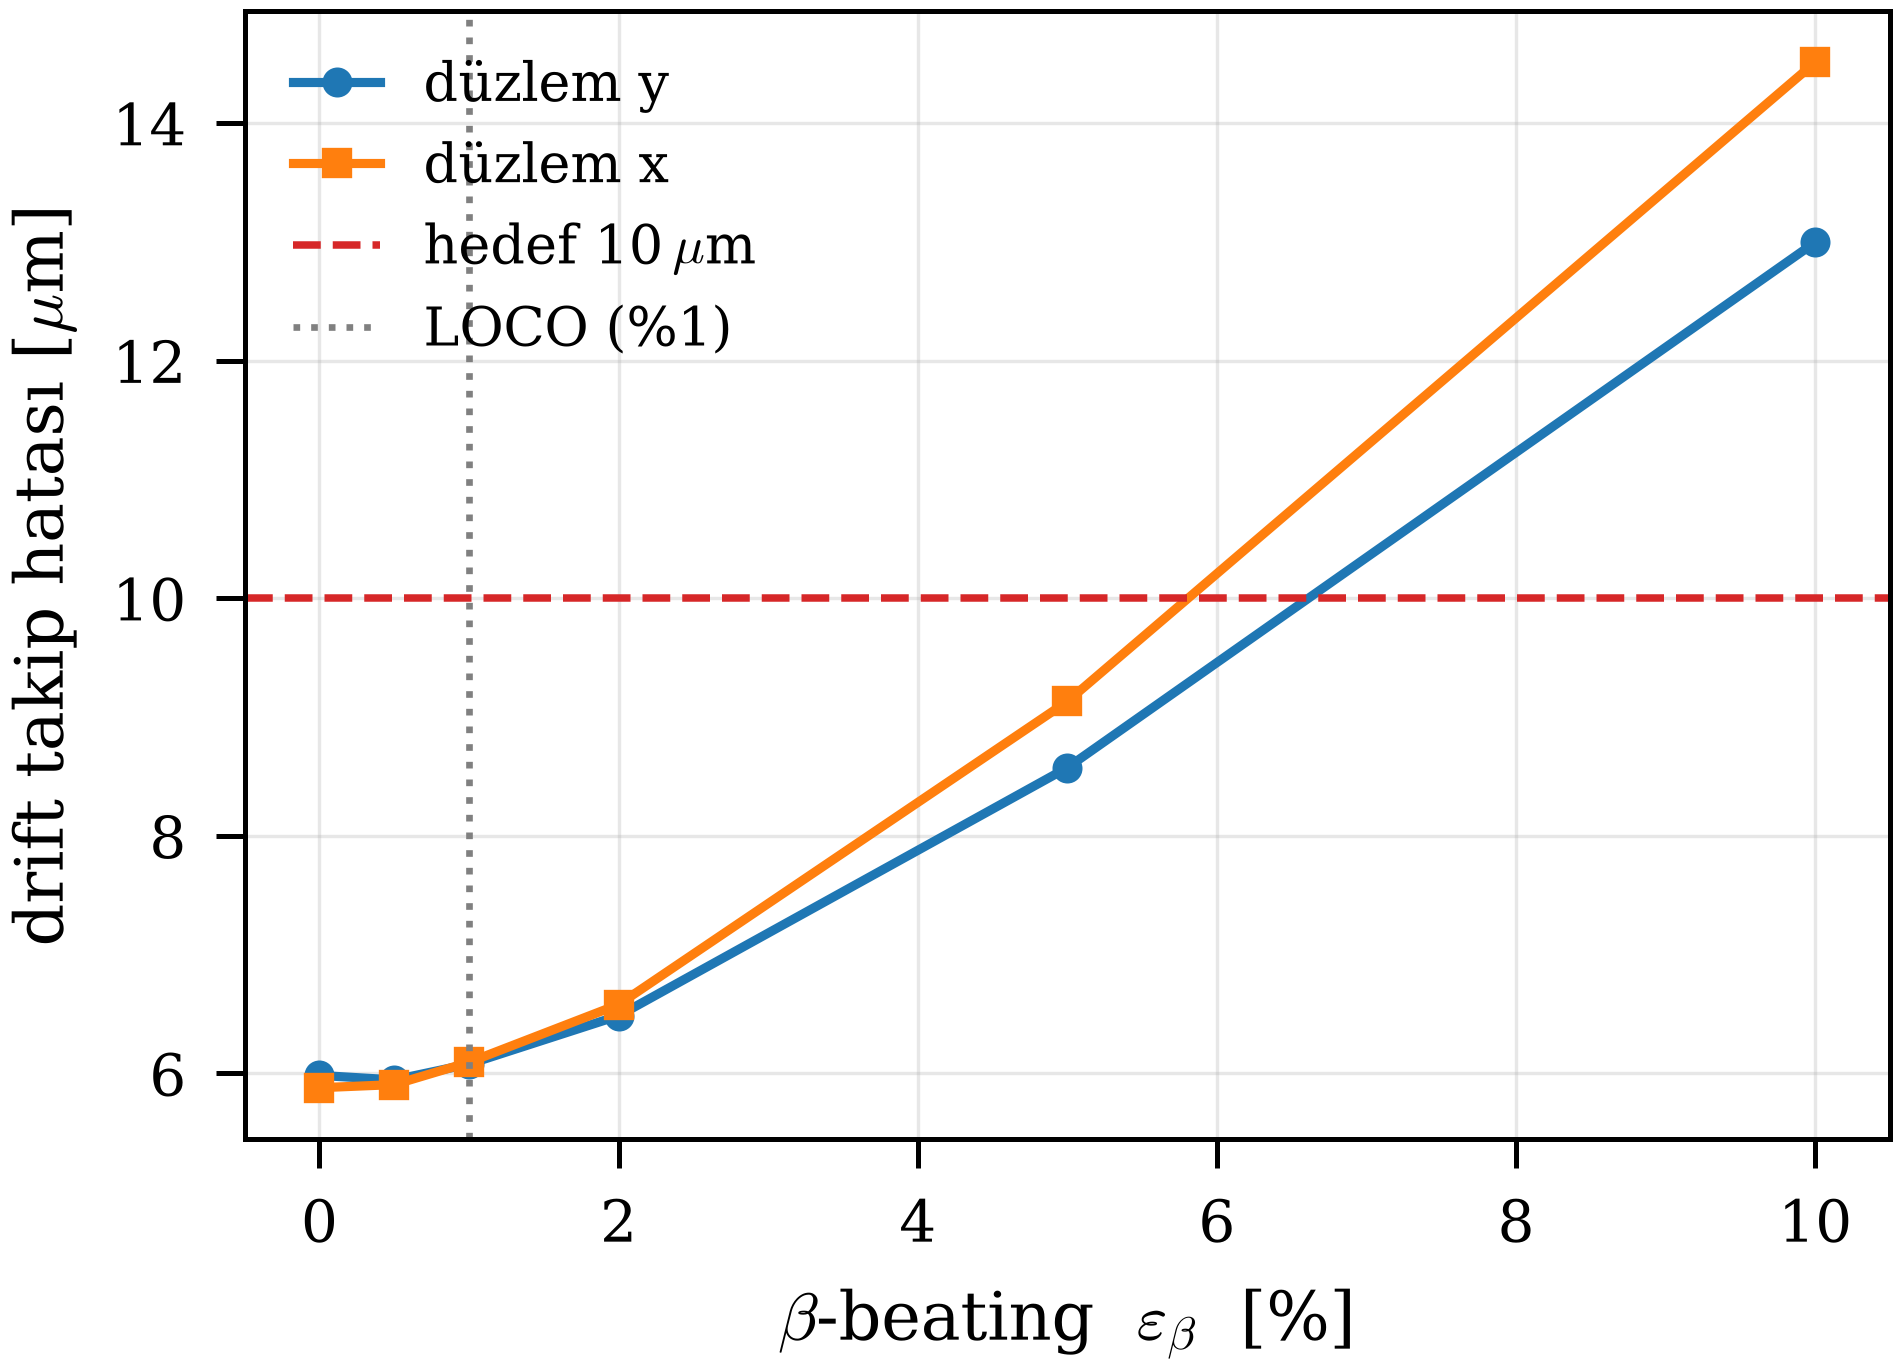
\includegraphics[width=\columnwidth]{fig3_betabeat.png}
\caption{Test 8: örgü-modeli hatası ($\beta$-beating) altında drift takip
hatası, $\varepsilon_\beta$'ya karşı (15-tohum medyanı). Kesik kırmızı çizgi
10\,$\mu$m hedef, noktalı gri çizgi LOCO-gerçekçi \%1 seviyesi. \%1'de hata
6.1\,$\mu$m; \%5'e kadar hedef altında.}
\label{fig:beta}
\end{figure}

\subsection{Test özeti}
Tablo~\ref{tab:summary} altı testin ana sayısını derler.

\begin{table*}[tb]
\centering
\caption{Sayısal deneylerin özeti.}
\label{tab:summary}
\begin{tabular}{@{}cll@{}}
\toprule
Test & Soru & Ana sayı \\
\midrule
1 & Düzenlileştirme $\Delta R$'yi kurtarır mı? & $1865\to52\,\mu$m, ama direct $3.5\,\mu$m \\
2 & Düzenlileştirme nasıl çuvallıyor? & 48 modun 43--45'i siliniyor \\
3 & Yatay modelde ters-suç? & $\pm10\%\to{<}0.5\,\mu$m \\
4 & Drift modu ofseti tolere eder mi? & $197\,\mu$m $\to$ $6.6\,\mu$m ($29\times$) \\
5 & Ofset kayarsa? & $<2\,\mu$m/epoch'a kadar üstün \\
6 & Aday yöntemler yan yana? & $\Delta R$: 1000--3700\,$\mu$m, drift: 6--7\,$\mu$m \\
8 & $\beta$-beating? & \%1$\to$6.1\,$\mu$m; \%5$\to$8.6\,$\mu$m; hedef altında \\
\bottomrule
\end{tabular}
\end{table*}

% ============================================================
\section{Gözlenebilirlik Sınırı}
Bu bölüm yöntemin \textbf{hangi hizalama desenlerini} iyi, hangilerini kötü
çözdüğünü karakterize eder. Bu, drift modunun gürültü tabanının (\S3) rastgele
bir sayı olmadığını; tepki matrisinin mod yapısından kaynaklanan, yöntemin
geçerlilik alanını ve kör noktasını tanımlayan yapısal bir özellik olduğunu
gösterir. (Bu karakterizasyon tümüyle monitörün kendi özelliğidir; herhangi bir
fiziksel sistematik bütçesinden bağımsız geçerlidir.)

\subsection{Hangi kaçıklık desenleri kapalı yörüngede görünür?}
Önce kurulumu somutlaştıralım. Halka 24 FODO hücresinden oluşur; her hücrede bir
\textbf{odaklayıcı} kuadrupol (QF) ve bir \textbf{dağıtıcı} kuadrupol (QD)
vardır --- toplam 48 kuadrupol. Bir ``hizalama hatası deseni'', 48 kuadrupolün
dikey kaymalarını veren 48 sayılık bir vektördür ($\Delta q\in\mathbb{R}^{48}$).
Bir kaymış kuadrupolün kapalı yörüngeye etkisi bir \textbf{kick}tir (küçük açısal
sapma) ve büyüklüğü (gradyan $\times$ kayma) ile orantılıdır.

Bir kick dizisinin kapalı yörüngeye toplam etkisi, kick deseninin \textbf{azimutal
harmoniğine} --- halka çevresi boyunca kaç kez tekrarladığına, $k$ --- bağlıdır.
Kapalı yörünge harmonik $k$'ya bir kazançla yanıt verir:
\begin{equation}
G_k = \frac{C}{\,|Q_\text{eff}^2-k^2|\,},\quad C\approx 24.8,\;
Q_\text{eff}^2\approx 5.03,
\label{eq:gain}
\end{equation}
burada $Q$ betatron tune'udur ($\approx 2.7$); sabitler bu örgüye özgüdür.
Kazanç tune'a yakın ($k\approx Q$) harmoniklerde en büyük, $k\gg Q$
harmoniklerde küçüktür. Yani \textbf{kapalı yörünge bir mod-seçici (rezonant)
filtredir}: yalnız belirli uzaysal harmonikleri güçlü gösterir. (Bu klasik bir
alçak-geçiren filtre değildir --- tepe $k=0$'da değil $k\approx Q$'dadır.)

\subsection{İki tür hizalama deseni: simetrik ve antisimetrik}
Hangi desenin hangi harmoniğe düştüğünü görmek için hizalama hatalarını
hücre-hücre iki gruba ayırıyoruz. Her hücredeki (QF, QD) çifti için iki uç durum:
\begin{itemize}
\item \textbf{Antisimetrik desen:} QF ve QD \textbf{zıt yönde} kayar
  (ör.\ QF $+a$, QD $-a$).
\item \textbf{Simetrik desen:} QF ve QD \textbf{aynı yönde} kayar
  (QF $+a$, QD $+a$).
\end{itemize}
Her hizalama hatası bu ikisinin toplamı olarak yazılabilir; böylece 48-boyutlu
desen uzayı iki dik \textbf{alt-uzaya} ayrılır (her biri 24-boyutlu). Buradaki
``alt-uzay'' basitçe \emph{belli bir simetri kuralına uyan tüm desenlerin
ailesi} demektir.

Belirleyici ayrıntı \textbf{gradyan işaretidir}: QF odaklar (gradyan $+$), QD
dağıtır (gradyan $-$). Kick $=$ gradyan $\times$ kayma olduğundan:
\begin{itemize}
\item \textbf{Antisimetrik} (kaymalar $+a/-a$, gradyanlar $+/-$): iki kick
  \textbf{aynı işarette} toplanır $\rightarrow$ düzgün, \textbf{düşük-$k$} desen
  $\rightarrow$ $G_k$ büyük $\rightarrow$ \textbf{yörüngede görünür}.
\item \textbf{Simetrik} (kaymalar $+a/+a$, gradyanlar $+/-$): iki kick
  \textbf{zıt işarette} $\rightarrow$ hücre içinde işaret değiştiren, hızlı
  alternatif \textbf{yüksek-$k$ ($k\approx 24$)} desen $\rightarrow$ $k\gg Q$
  $\rightarrow$ $G_k$ küçük $\rightarrow$ \textbf{yörüngede neredeyse görünmez}.
\end{itemize}
Sezgi: simetrik kayma, gradyan alternasyonu yüzünden kendi kendini söndüren bir
kick örüntüsü üretir; kapalı yörünge bunu ``görmez'', antisimetrik kaymayı ise
güçlü görür.

\subsection{Hangi desenler ne kadar gürültüyle kestirilir? (per-mod SVD)}
\S4.2'deki simetrik/antisimetrik ayrım kategorikti (iki uç durum). Tepki
matrisinin \textbf{tekil değer ayrışımı (SVD)} bunu nicel ve sürekli hale
getirir. $R=U\Sigma V^\top$ yazıldığında her sağ-tekil vektör $V_i$ bir hizalama
deseni (``mod''), karşılık gelen tekil değer $\sigma_i$ ise o desenin yörüngede
ne kadar güçlü göründüğüdür; monitör o modu kestirirken gürültüyü $1/\sigma_i$
ile büyütür. Her mod için gürültü büyütmesi $1/\sigma_i$ ve modun \S4.2 anlamında
simetrik içeriği hesaplanır ($\sigma_{\max}=28.4$, $\sigma_{\min}=0.147$,
$\kappa(R)=193$; Tablo~\ref{tab:svd}). En iyi 8 mod ortalama \textbf{\%4} simetrik (antisimetrik
baskın, iyi koşullu); en kötü 8 mod ortalama \textbf{\%96} simetrik. En kötü
modun ($\sigma_{\min}$) koşulluluk-kaynaklı duyarlılığı en iyiye göre
$\sim 193$ kat ($=\kappa(R)$) daha kötüdür; bu fark tümüyle simetrik
alt-uzayda yoğunlaşır. (Bu, ``tüm simetrik modlar 193 kat kötü'' demek
değildir; tablodaki $1/\sigma$ sütunu mod-mod artışı gösterir.) Bu ilişki
Şekil~\ref{fig:permode}'te açıkça görülür: gürültü duyarlılığı $1/\sigma$
arttıkça simetrik güç oranı \%100'e tırmanır.

\begin{table}[tb]
\centering\small
\caption{Seçili singüler modlar: gürültü duyarlılığı ve simetrik içerik.}
\label{tab:svd}
\begin{tabular}{@{}rrrr@{}}
\toprule
Mod & $\sigma$ & $1/\sigma$ & Sim. güç \\
\midrule
0 (en iyi)  & 28.4  & 0.04 & \%4 \\
2           & 10.1  & 0.10 & \%6 \\
10          & 2.0   & 0.51 & \%13 \\
20          & 0.49  & 2.03 & \%42 \\
40          & 0.16  & 6.39 & \%91 \\
47 (en kötü)& 0.147 & 6.82 & \textbf{\%98} \\
\bottomrule
\end{tabular}
\end{table}

\begin{figure}[tb]
\centering
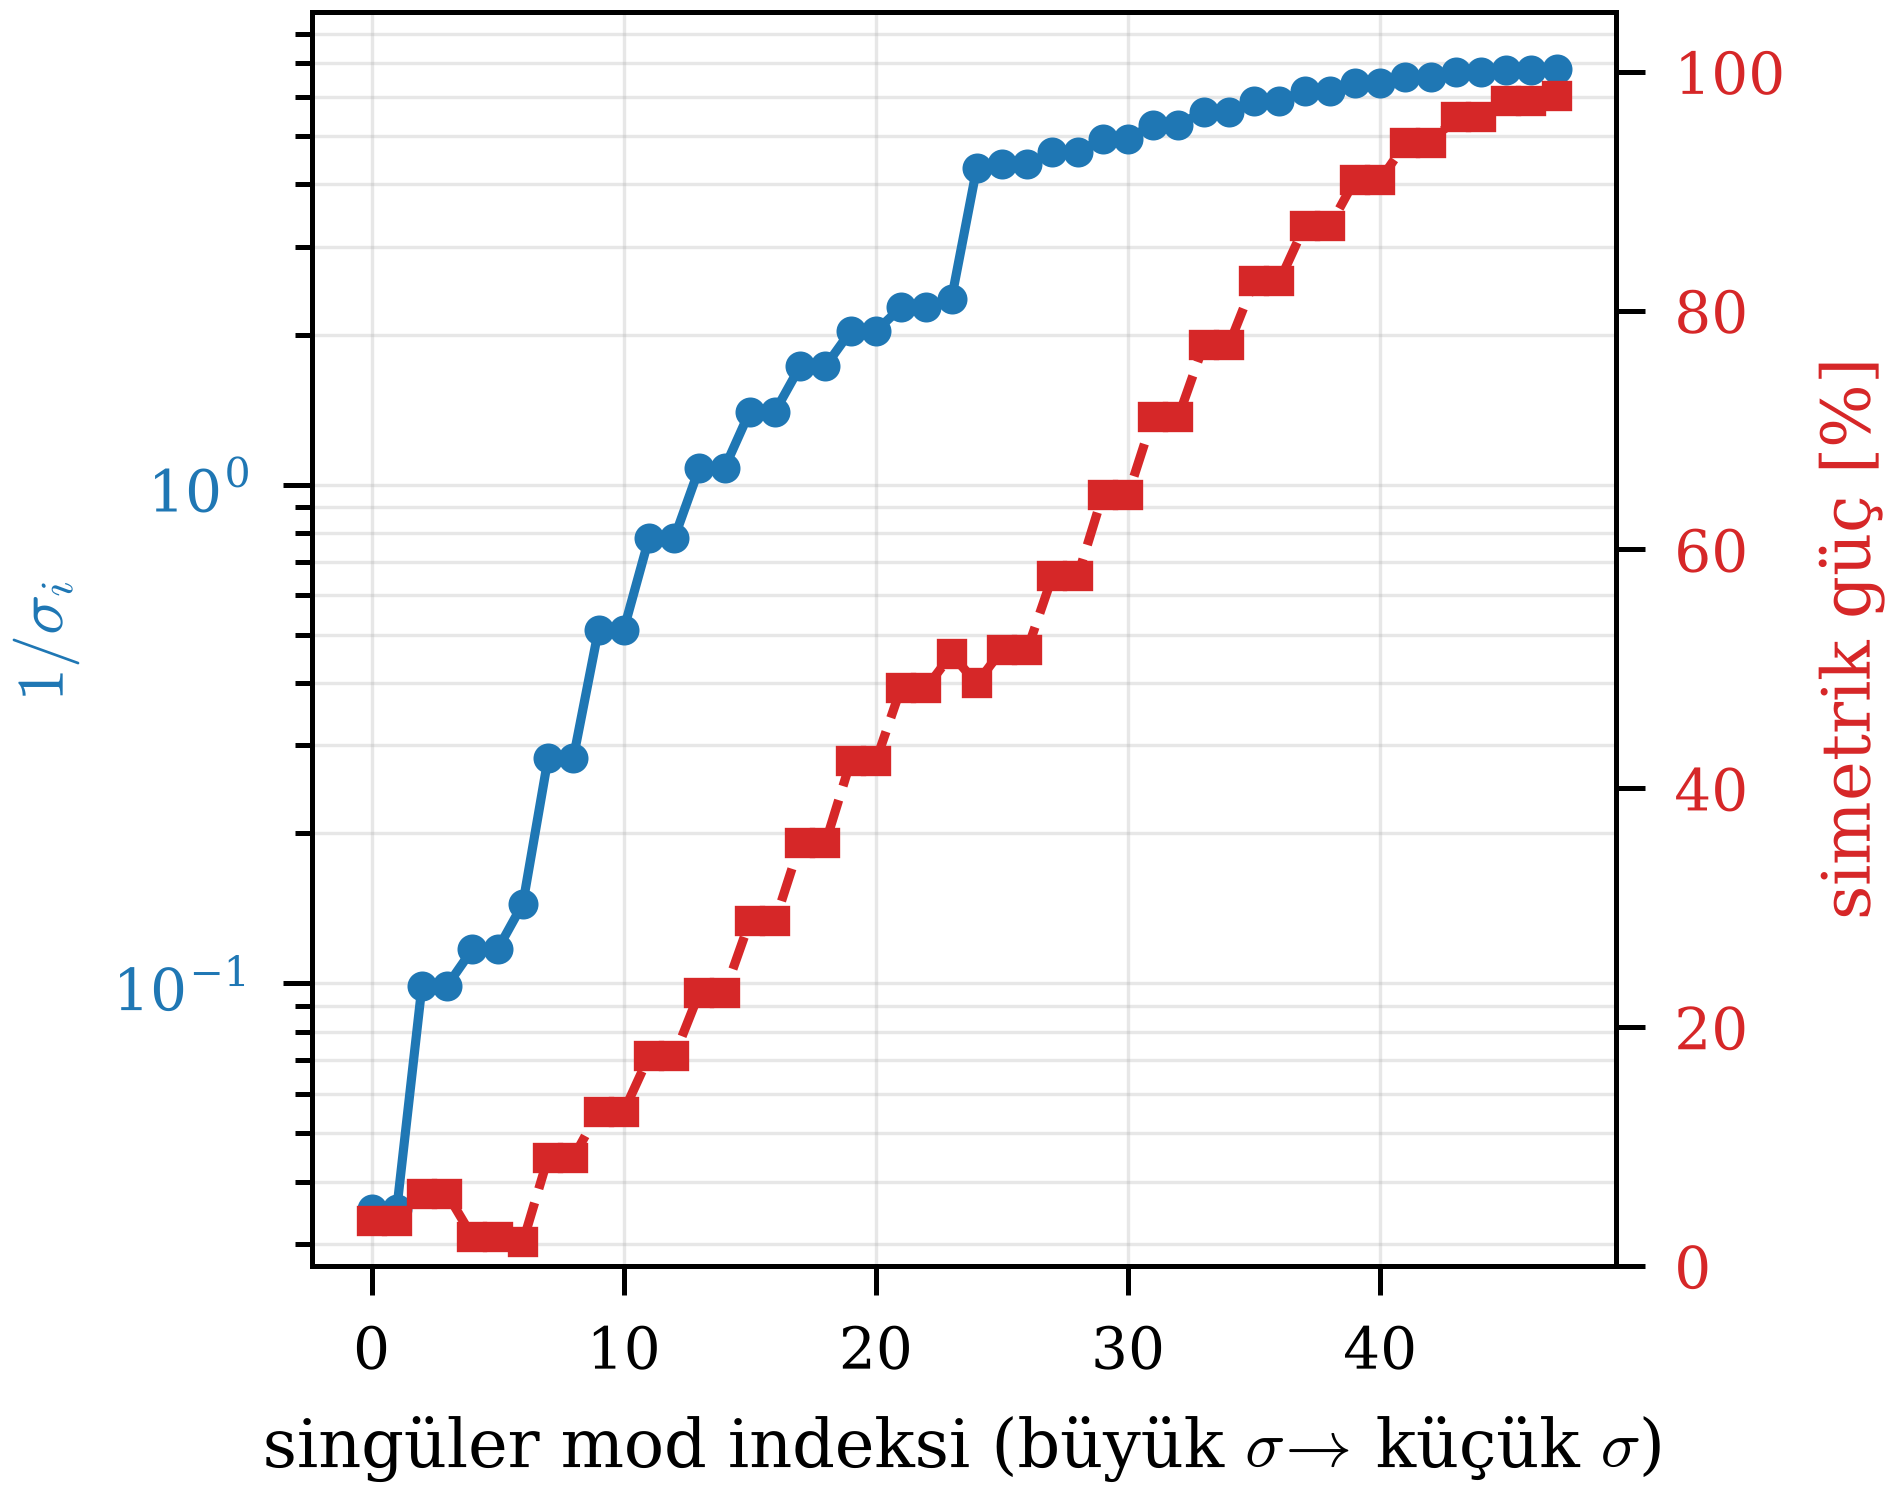
\includegraphics[width=\columnwidth]{fig4_permode_svd.png}
\caption{$R$'nin (dikey düzlem) singüler modları: sol eksen (mavi) gürültü
duyarlılığı $1/\sigma_i$, sağ eksen (kırmızı) modun simetrik alt-uzaydaki güç
oranı. En kötü koşullanmış modlar (sağ) \%96--98 simetriktir; gürültü
duyarlılığı arttıkça simetrik içerik \%100'e tırmanır.}
\label{fig:permode}
\end{figure}

\subsection{Kör noktanın anlamı ve sistematik bütçeyle ilişkisi (ileri bakış)}
\S4.1--4.3'ün sonucu \textbf{yöntem düzeyinde} kesin bir ifadedir: kapalı-yörünge
drift monitörü antisimetrik hizalama driftini güçlü, simetrik driftini ise
$\sim 193$ kat daha gürültülü çözer. Bu, monitörün geçerlilik alanını
(antisimetrik) ve kör noktasını (simetrik) tanımlar ve daha iyi BPM donanımı ya
da daha fazla veriyle kapanmaz; bu alt-uzaya erişim ilkesel olarak
\textbf{farklı bir gözlemlenebilir} (ör.\ karşı-dönen CW/CCW demet ayrımı veya
doğrudan spin presesyonu \cite{omarov2022}) gerektirir.

Bu kör noktanın belirli bir \textbf{sistematik bütçe} için ne kadar önemli
olduğu ayrı bir sorudur. pEDM bağlamında ilgili sistematik, kaçıklığın ürettiği
sahte EDM'dir; baskın kanalı yatay$\times$dikey kaçıklığın çarpımına
($dx\cdot dy$) bağlı, misalignment'ta ikinci-dereceden bir geometrik-faz
etkisidir \cite{omarov2022}. Bu kanalın ağırlığının monitörün zayıf-gözlediği
simetrik alt-uzaya ne kadar düştüğü desen-bağımlı, inceliklidir ve tek bir
kapalı-yörünge ölçümüyle çözülemez. Bu nedenle sahte-EDM $\leftrightarrow$
gözlenebilirlik bağını niceleme işini --- tam parçacık + spin izleyicisiyle,
orbit-düzeltme öncesi/sonrası ayrımıyla --- \textbf{bu çalışmanın kapsamı
dışında, ayrı bir incelemeye} bırakıyoruz. Bu makalenin iddiası yöntem düzeyinde
kalır: monitör, antisimetrik hizalama driftini ucuza ve sürekli izleyen,
geçerlilik alanı ve kör noktası net tanımlı bir araçtır.

% ============================================================
\section{Önerilen İşletme Modu}
Tek bir yöntem her ihtiyacı karşılamaz; iki katmanlı bir mimari öneriyoruz
(Şekil~\ref{fig:mimari}).

\paragraph{Yavaş mutlak katman (saatlik--günlük).} LOCO \cite{safranek1997} +
BBA + survey ile mutlak hizalama $\Delta q_0$, BPM ofseti $\mathbf{b}_0$ ve örgü modeli
($\beta,\phi,Q$, dolayısıyla $R$). Bu, hızlandırıcı operasyonunda zaten var
olan standart prosedürdür.

\paragraph{Hızlı drift katmanı (sürekli, saniye--dakika).} Bu çalışmanın
katkısı: $\widehat{\delta q}(t)=R^{-1}(\mathbf{y}(t)-\mathbf{y}_0)$. Fizik
run'ı boyunca sürekli çalışır, veri toplamayı bozmaz, kalibrasyondan beri
(antisimetrik) hizalama değişimini izler.

İki katman tamamlayıcıdır: yavaş katman mutlak referansı ve $R$'yi sağlar,
hızlı katman o referansa göre değişimi takip eder. \S4'ün sınırı gereği, her
iki katman da simetrik alt-uzayı kapalı yörüngeden kurtaramaz; bu bilgi dış
bir gözlemlenebilirden (demet ayrımı / spin) gelmelidir.

\begin{figure}[tb]
\centering
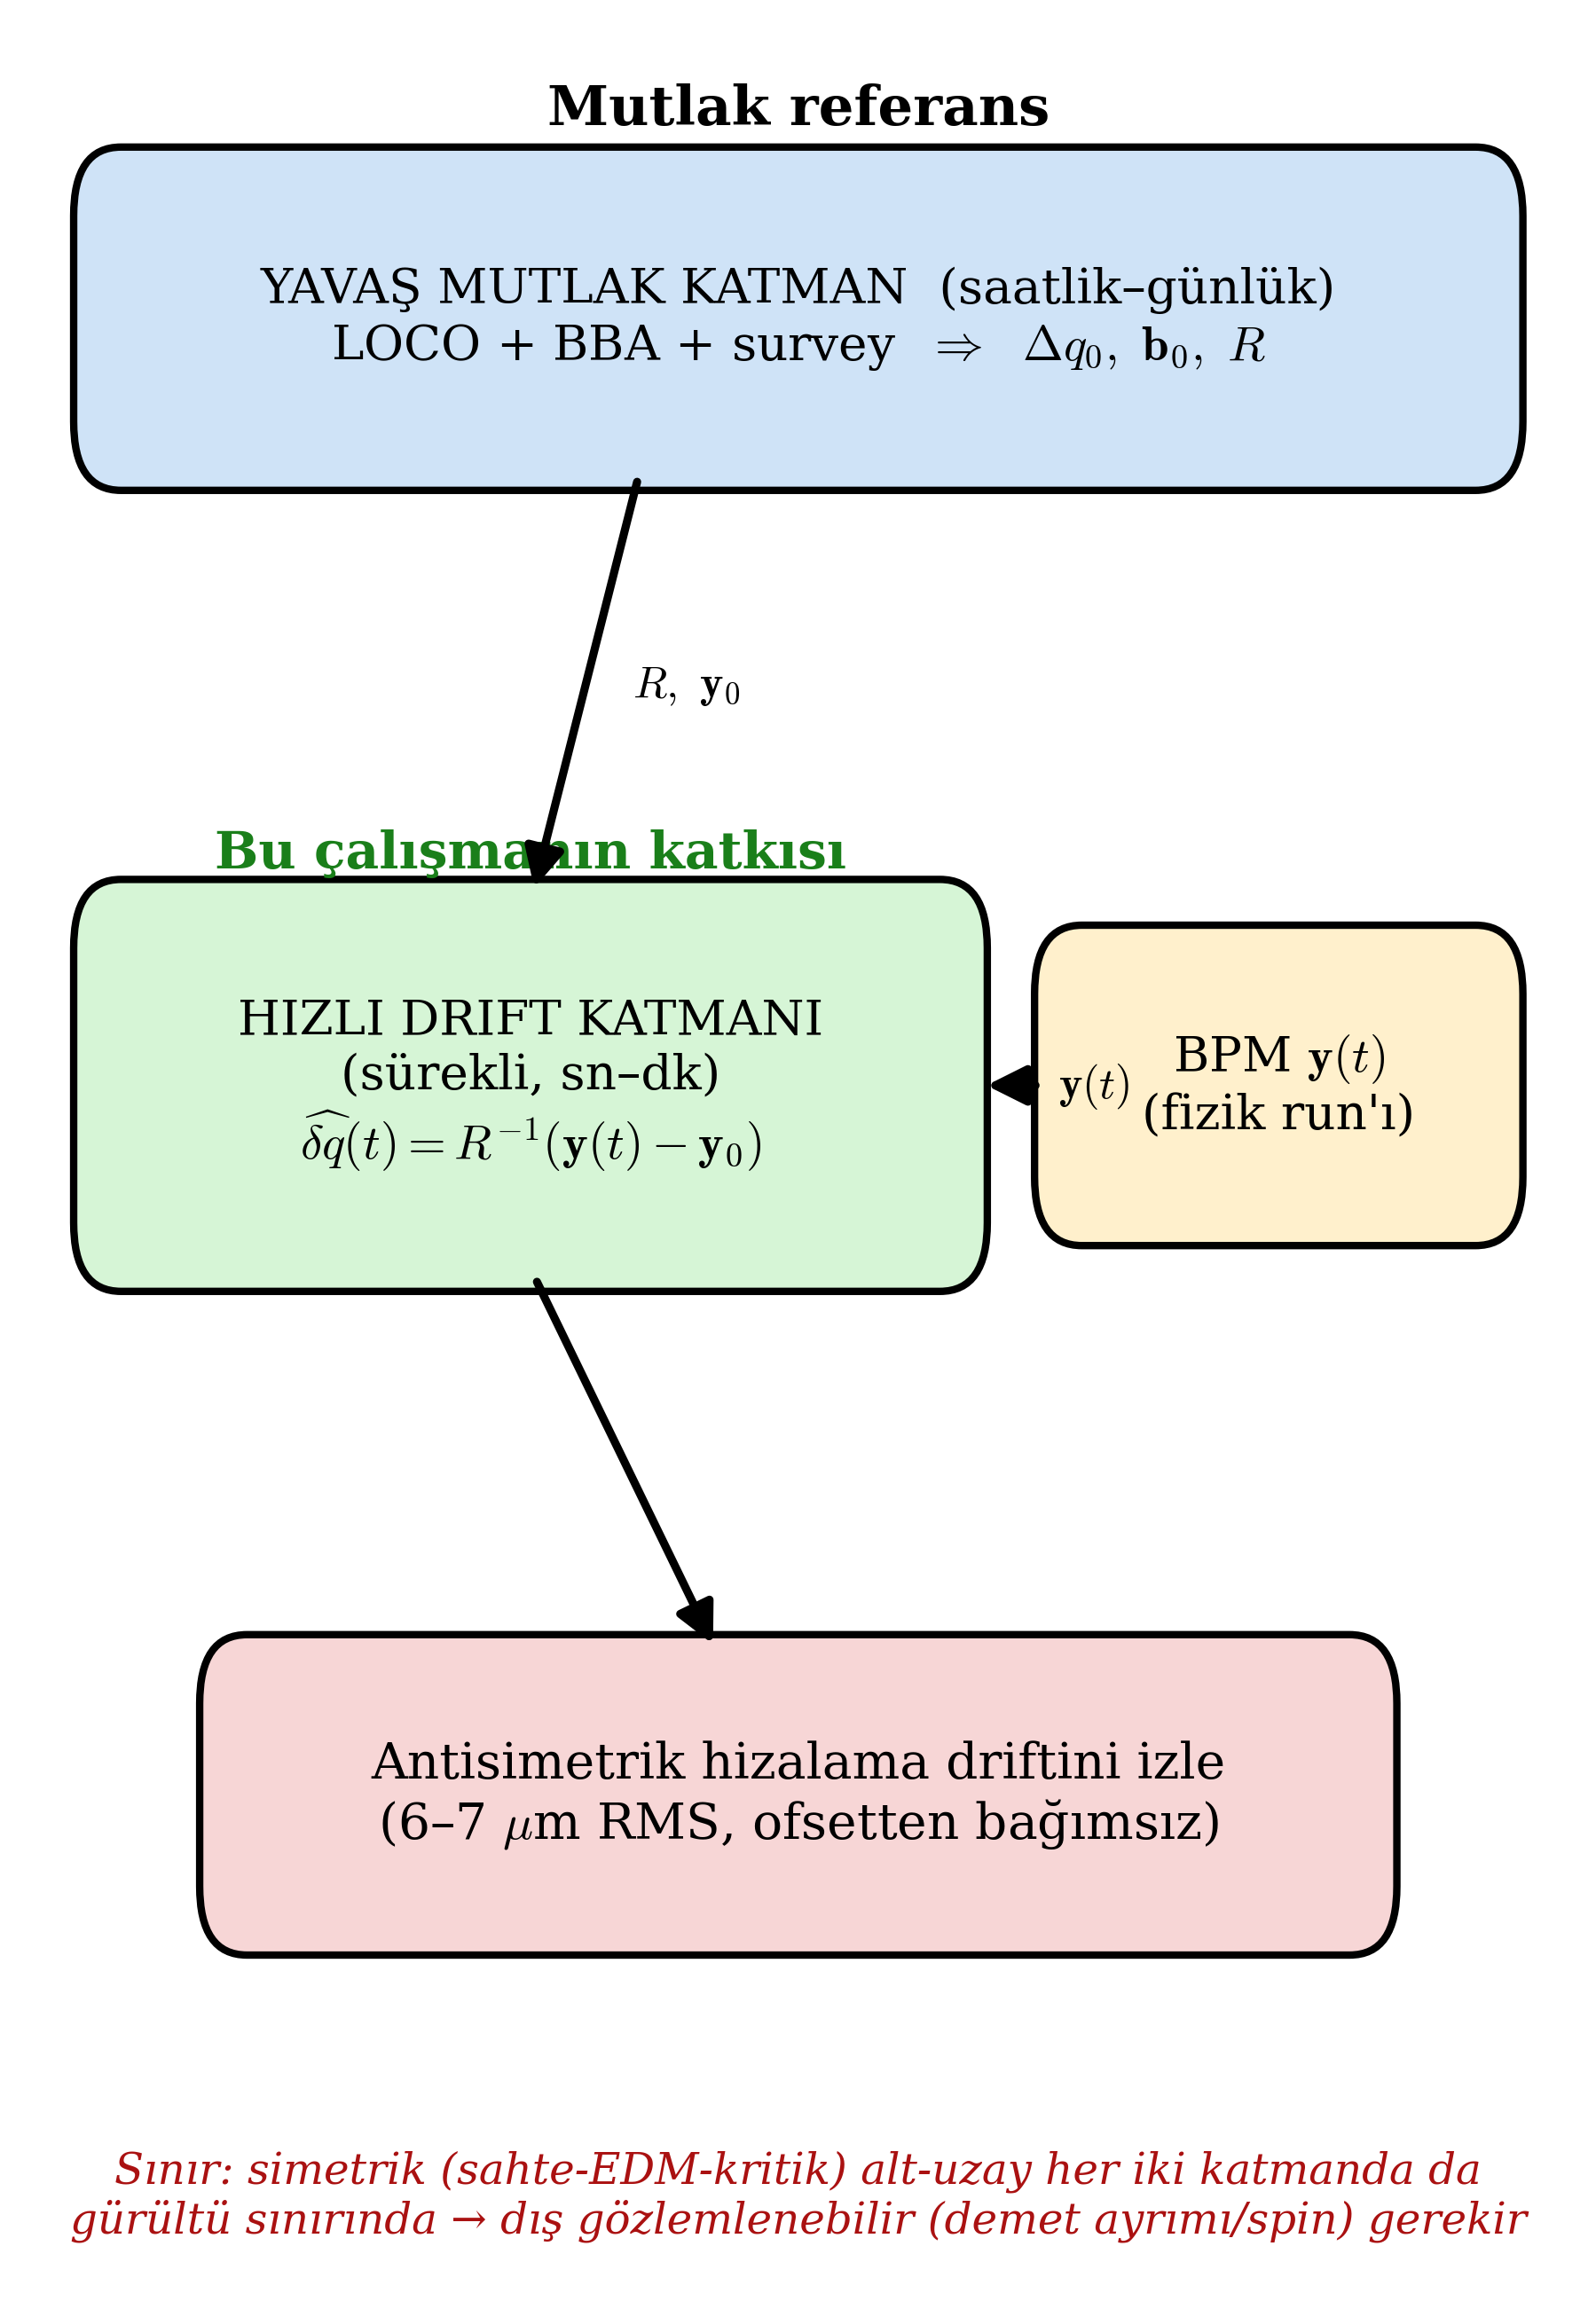
\includegraphics[width=\columnwidth]{fig5_mimari.png}
\caption{İki-katmanlı hizalama izleme mimarisi: yavaş mutlak katman
(LOCO/BBA $\rightarrow \Delta q_0,\mathbf{b}_0,R$) ve hızlı drift katmanı
($R^{-1}(\mathbf{y}(t)-\mathbf{y}_0)$). Simetrik (sahte-EDM-kritik) alt-uzay
her iki katmanda da gürültü sınırındadır.}
\label{fig:mimari}
\end{figure}

% ============================================================
\section{Tartışma ve Sonuç}
Bu çalışmada pEDM AG halkasında kuadrupol hizalama driftini sürekli izlemek
için kalibrasyon-referans yöntemi önerildi ve gerçekçi BPM hata bütçesi
altında (50\,$\mu$m ofset, 1\,$\mu$m gürültü, 0.2\,mrad tilt) 6--7\,$\mu$m RMS
hassasiyetle, $\sim$\%1 $\beta$-beating'e dayanıklı şekilde çalıştığı
sistematik testlerle gösterildi. Yöntem iki katmanlı bir mimaride (yavaş
LOCO/BBA + hızlı drift) operasyonel olarak konumlandırıldı.

Yöntemin \textbf{gözlenebilirlik sınırı} da nicelendi (\S4): per-mod SVD
analizi, monitörün kör noktasının \%96 simetrik içerikli en kötü koşullanmış
modlar olduğunu gösterir (en kötü modda en iyiye göre $\sim 193$ kat duyarlılık
dezavantajı). Yani monitör antisimetrik hizalama driftini hassasça izler;
simetrik drift yöntemin geçerlilik alanı dışındadır ve donanım/veriyle kapanmayan
yapısal nedenlerle erişimi farklı bir gözlemlenebilir gerektirir. Bu kör noktanın
belirli bir sistematik bütçe (ör.\ kaçıklığın ürettiği sahte EDM) için önemi
makineye bağlı, ayrı bir sorudur ve bu çalışmanın kapsamı dışındadır (\S4.4).

Çalışmanın kısıtları:
\begin{itemize}
\item \textbf{Lineer model ötesi.} Sonuçlar Eş.~\eqref{eq:lin}'e dayanır;
  gerçek halkada BPM gain hataları, roll/kuplaj, sekstupol feed-down, fringe
  alanlar, histerezis ve akım dalgalanması vardır. Bunların sistematik
  incelenmesi gelecek çalışmadır.
\item \textbf{Tek kafes.} Tüm sonuçlar 24-hücreli FODO'da. Genellenebilirlik
  kazanç yasası $G_k$ üzerinden tahmin edilebilir ama doğrulanmamıştır.
\item \textbf{BPM ofset kararlılığı operasyonel bir gerekliliktir.} Yöntem BPM
  ofsetine \emph{duyarsız} değildir; ofsetin \emph{hızına} duyarsızdır. Drift
  modu $\mathbf{b}(t)\approx\mathbf{b}_0$ varsayar ve geçerliliği bir
  kayma-hızı bütçesine bağlıdır: $\dot{\mathbf{b}}\lesssim 2\,\mu$m/epoch
  (\S3.5). Bu eşiğin pEDM BPM donanımında saatler--günler ölçeğinde sağlanıp
  sağlanmadığı deneysel olarak karakterize edilmelidir; yöntemin pratik
  kullanılabilirliğinin belirleyicisidir.
\end{itemize}

% ============================================================
\appendix
\section{Sayısal simülasyon altyapısı}
Tüm sonuçlar Python tabanlı bir altyapıda üretildi. Parçacık takibi
dördüncü-mertebe Gauss-Legendre (GL4) semplektik integratörüyle; analitik tepki
matrisi Courant-Snyder formalizmiyle (\texttt{fodo\_lattice.py}) inşa edildi.
Ana gösterim \texttt{drift\_monitor\_sim.py} (Test~4), $\beta$-beating
sağlamlığı \texttt{test8\_betabeat.py} (Test~8), per-mod SVD analizi
\texttt{permode2.py} içindedir. Şekiller \texttt{make\_figures.py} (Şekil 1--4,
6) ve \texttt{make\_fig5\_architecture.py} (Şekil 5) ile üretilir.

% ============================================================
\begin{thebibliography}{9}
\bibitem{omarov2022}
Z.~Omarov, H.~Davoudiasl, S.~Hac\i{}\"omero\u{g}lu, V.~Lebedev, W.~M.~Morse,
Y.~K.~Semertzidis, A.~J.~Silenko, E.~J.~Stephenson, and R.~Suleiman,
``Comprehensive symmetric-hybrid ring design for a proton EDM experiment at
below $10^{-29}\,e\cdot$cm,'' \emph{Phys.\ Rev.\ D} \textbf{105}, 032001
(2022),
\href{https://doi.org/10.1103/PhysRevD.105.032001}{doi:10.1103/PhysRevD.105.032001};
arXiv:2007.10332.
\bibitem{anastassopoulos2016}
V.~Anastassopoulos \emph{et al.}, ``A storage ring experiment to detect a
proton electric dipole moment,'' \emph{Rev.\ Sci.\ Instrum.} \textbf{87},
115116 (2016),
\href{https://doi.org/10.1063/1.4967465}{doi:10.1063/1.4967465};
arXiv:1502.04317.
\bibitem{lee2011}
S.~Y.~Lee, \emph{Accelerator Physics}, 3rd ed.\ (World Scientific, 2011),
\href{https://doi.org/10.1142/8335}{doi:10.1142/8335}.
\bibitem{safranek1997}
J.~Safranek, ``Experimental determination of storage ring optics using orbit
response measurements,'' \emph{Nucl.\ Instrum.\ Meth.\ A} \textbf{388}, 27
(1997),
\href{https://doi.org/10.1016/S0168-9002(97)00309-4}{doi:10.1016/S0168-9002(97)00309-4}.
\end{thebibliography}

\end{document}
